\documentclass[compress]{beamer}

\usepackage[nofonts]{ctex}
\setCJKmainfont[ItalicFont={Kaiti SC}]{Kaiti SC}%
%\setCJKmainfont[ItalicFont={AR PL KaitiM GB}]{AR PL KaitiM GB}%
%\setCJKsansfont{WenQuanYi Zen Hei}% 文泉驿的黑体

\mode<beamer>
{
     \useinnertheme{rectangles}
     %\useoutertheme{infolines}
     %\useoutertheme{split}
     \usecolortheme{rose}
     \usecolortheme{seahorse}

     \setbeamertemplate{navigation symbols}{}%remove navigation symbols

     %\expandafter\def\expandafter\insertshorttitle\expandafter{%
     %\insertshorttitle\hfill%
     %\insertframenumber\,/\,\inserttotalframenumber}
     %\raisebox{-1ex}{
\includegraphics[width=3ex]{Overlays/logo.pdf}}}
    \setbeamertemplate{footline} {
      \leavevmode%
      \hbox{%
      \begin{beamercolorbox}[wd=.1\paperwidth,ht=2.25ex,dp=1ex,left]{date in head/foot}%
        \usebeamerfont{date in head/foot}%
        \hspace*{1ex}\raisebox{-0.8ex}{
\includegraphics[width=3ex]{Overlays/logo.pdf}}%
      \end{beamercolorbox}%
      \begin{beamercolorbox}[wd=.4\paperwidth,ht=2.25ex,dp=1ex,right]{date in head/foot}%
        \usebeamerfont{date in head/foot}\insertsection\hspace*{1ex}
      \end{beamercolorbox}%
      \begin{beamercolorbox}[wd=.4\paperwidth,ht=2.25ex,dp=1ex,left]{date in head/foot}%
        \usebeamerfont{date in head/foot}\hspace*{1ex}\insertsubsection
      \end{beamercolorbox}%
      \begin{beamercolorbox}[wd=.1\paperwidth,ht=2.25ex,dp=1ex,right]{date in head/foot}%
        \insertframenumber{} / \inserttotalframenumber\hspace*{1ex}
      \end{beamercolorbox}}%
      \vskip0pt%
    }

}

%\defbeamertemplate*{footline}{mytheme}
%{
%  \leavevmode%
%  \hbox{%
%  \begin{beamercolorbox}[wd=.5\paperwidth,ht=2.25ex,dp=1ex,center]{author in head/foot}%
%    \usebeamerfont{author in head/foot}\insertshortauthor~~%
%    \raisebox{-1ex}{
\includegraphics[width=3ex]{Overlays/logo.pdf}}%
%  \end{beamercolorbox}%
%  \begin{beamercolorbox}[wd=.5\paperwidth,ht=2.25ex,dp=1ex,right]{title in head/foot}%
%    \usebeamerfont{title in head/foot}\insertshorttitle{}\hspace*{2em}
%    \insertframenumber{} / \inserttotalframenumber\hspace*{2ex} 
%  \end{beamercolorbox}}%
%  \vskip0pt%
%}
%\usebeamertemplate{mytheme}

%\setbeamercovered{transparent}

\mode<handout>
{
	\usetheme{default}
	\usepackage{pgfpages}
	\pgfpagesuselayout{4 on 1}[a4paper,landscape,border shrink=5mm]
}


\usepackage{amsmath,latexsym,amssymb,amsfonts,amsbsy}
\usepackage{graphicx}
\usepackage{hyperref}
\usepackage{ulem}
\usepackage{fancyvrb}
\fvset{frame=single, numbers=left, fontsize=\small}
\usepackage{comment}

\usepackage{tikz}
\usetikzlibrary{calc,arrows.meta, graphs, trees, shapes, positioning,
shapes.geometric, shapes.multipart, patterns}
\usepackage{tikz-uml}


\newcommand{\romannumber}[1]{{\textrm{\uppercase\expandafter{\romannumeral
#1}}}}

\newcommand{\textblue}[1]{\textcolor{blue}{#1}}

\setbeamercolor{dblue}{fg=white,bg=gray!70!blue} % for beamercolorbox
 \newenvironment{pblock}{\begin{beamercolorbox}[rounded=true,
          shadow=false]{dblue}}{\end{beamercolorbox}}
 \newenvironment{bblock}{\begin{beamercolorbox}[rounded=true,
          shadow=false]{fg=black, bg=white}}{\end{beamercolorbox}}

\graphicspath{{figure/}}

%%%%%%%%%%%%%%%%%%%%%%%%%%%%%%%%%%%%%%%%%%%%%%%%%%%%%%%%%%%%%%%%%
%    body                                                       %
%%%%%%%%%%%%%%%%%%%%%%%%%%%%%%%%%%%%%%%%%%%%%%%%%%%%%%%%%%%%%%%%%


\begin{document}

\AtBeginSubsection[]
{ 
    \begin{frame}<beamer> 
		\frametitle{内容提要} 
		\tableofcontents[currentsection,currentsubsection,
        subsectionstyle=show/shaded/hide] 
	\end{frame} 
} 

					
\title{第三章 ~~ 建立需求模型, 定义对象类}

\author[面向对象的分析与设计]
{曹东刚\\\href{mailto:caodg@pku.edu.cn}{caodg@pku.edu.cn}}

\institute[北京大学]{北京大学信息学院研究生课程 - 面向对象的分析与设计 \\
\href{http://sei.pku.edu.cn/~caodg/course/oo}{http://sei.pku.edu.cn/\~{}caodg/course/oo}}

\date{}

\titlegraphic{
\includegraphics[height=0.1\textwidth]{Overlays/logo.pdf}}

%\includeonlyframes{current}

\begin{frame}[plain]
	\titlepage
\end{frame}

\setcounter{framenumber}{0}

\section{建立需求模型}

\subsection{需求分析}

\begin{frame}
  \frametitle{需求分析和系统分析}
  \begin{block}{需求分析}
    对用户需求进行分析,旨在产生一份明确、规范的需求定义
  \end{block}
  \begin{block}{面向对象的系统分析}
    把问题域中的事物抽象为系统中的对象,建立一个用面向对象概念表达的系统
    模型
  \end{block}
\end{frame}

\begin{frame}
  \frametitle{需求分析和面向对象的系统分析: 用况}
  \begin{block}{需求分析}
  需求分析的确切含义是对用户需求进行分析, 旨在产生一份明确、规范的需求定义
\end{block}

\vspace*{2ex}
\noindent\scalebox{0.8} {
    \begin{tikzpicture}
    \node [ellipse, draw, minimum width=4cm, text width=3cm, align=center] (Problem) {问题域 \\ (抽象的来源)} ; 
    \node [rectangle, draw, minimum width=3cm, text width=2cm, align=center, above right=2cm of Problem] (OOA) {OOA模型 \\ (类图)} ; 
    \node [cloud callout, draw, callout relative pointer={(3.5,-1)}, text width=3cm, aspect=3, cloud puffs=15, callout pointer segments=4, inner sep=0pt, align=center, above left=2cm of Problem] (Goal) {系统责任 \\ (抽象的目标)} ; 

    \node [single arrow, draw, above right=0.6cm of Problem.north east, rotate=30, inner sep=1pt, minimum height=2cm] {抽象} ;

    \pause

    \node [rectangle callout, draw, callout relative pointer={(0.6, -0.6)}, text width=2cm, fill=lime!60, align=center, above = 1.2cm of Problem] (Case) {需求模型 \\ (用况图)} ;

    \node [single arrow, draw, left=0.1cm of Case, inner sep=2.5pt, minimum height=1cm, fill=lime!60] {} ;
    \node [single arrow, draw, right=0.1cm of Case, inner sep=2.5pt, minimum height=1.5cm, fill=lime!60] {} ;

    \end{tikzpicture}
}
\end{frame}


\begin{frame}
  \frametitle{问题与思路}
  \begin{block}{问题的提出}
  在系统尚未存在时,如何描绘用户需要一个什么样的系统?\\
  如何规范地定义用户需求?
\end{block}

\begin{block}{解决的思路}
  针对问题域, 在系统责任的约束下, 把系统看作一个黑箱,看它对外部的客观世界发挥什么作用,
  描述其外部可见的行为
\end{block}
\end{frame}

\begin{frame}
    \frametitle{深刻认识问题域}
    \begin{itemize}
        \item 问题域的主要业务概况
        \item 要建设系统的业务目标
        \item 确定系统的涉众(Stakeholder)
        \item 规划要建设系统的业务范围
    \end{itemize}
\end{frame}

\begin{frame}
    \frametitle{涉众分析}
    \begin{itemize}
        \item 寻找可能的涉众: 
            \begin{itemize}
                \item 出资方, 项目发起者, 业务管理人员, 业务操作人员
            , 项目承担方, 其他各利益相关方
             \end{itemize}
        \item 通过访谈等活动, 明确各涉众的角色、目标和期望, 进行归纳、分
            类、排序、分析、总结, 形成一份涉众分析报告
    \end{itemize}
\end{frame}

\begin{frame}
    \frametitle{规划业务范围}
    \begin{enumerate}
        \item[0] 首先,界定项目承担方的能力范围: 项目周期、投入、成
            本等
        \item[1]  规划业务目标, 可以根据实际情况协商取消、调整或补充业务目
            标
        \item[2] 对涉众及其目标进行分析规划, 合理确定系统相关的涉众, 调整涉众目
            标(期望)
        \item[3] 对业务范围进行分析, 初步确定各业务目标的优先次序
        \item[4] 按照先整体再局部、先架构再流程的次序, 建立对业务范围的
            完整认识
    \end{enumerate}
\end{frame}

\begin{frame}
  \frametitle{系统边界}
  \begin{block}{系统边界}
    一个系统所包含的所有系统成分与系统以外各事物的分界线
  \end{block}
  \begin{block}{系统}
    被开发的计算机软硬件系统,不是指现实系统
  \end{block}
  \begin{block}{系统成分}
    在OOA和OOD中定义并且在编程时加以实现的系统元素——对象
  \end{block}

\end{frame}

\begin{frame}
    \frametitle{确定系统边界的依据}

    系统边界主要根据系统责任(目标)确定, 每个目标都有一个自己的边界 \\[2ex]

    思考: 和按功能或按模块划分边界相比,有何不同结果?

\end{frame}

\begin{frame}
  \frametitle{系统边界与参与者}

\noindent\begin{tikzpicture}

\renewcommand\baselinestretch{1.0}

\node[ellipse, draw, very thick, pattern=dots, minimum width=5cm, minimum height=3cm] (System) {} ;

\node [rectangle callout, rounded corners, draw, callout relative pointer={(0.5, -0.5)}, text width=3cm, text=blue, align=center, above left= 0.5cm of System] (N1) {系统是由一条边界包围起来的未知空间} ;

\pause

\node [double arrow, draw, inner sep=2pt, minimum height=0.8cm, rotate=45, fill=lime!60, double arrow head extend=4pt ] at (System.south west) {} ;
\node [double arrow, draw, inner sep=2pt, minimum height=0.8cm, rotate=90, fill=lime!60, double arrow head extend=4pt ] at (System.north) {} ;
\node [double arrow, draw, inner sep=2pt, minimum height=0.8cm, rotate=0, fill=lime!60, double arrow head extend=4pt ] at (System.east) {} ;
\node [rectangle callout, rounded corners, draw, callout relative pointer={(0.4, 0.3)}, text width=3cm, text=blue, align=center, below left= 0.5cm of System] (N1) {只通过有限的几个接口与外部交互} ;

\pause

\umlactor[x=-1.5, y=-2]{参与者}
\umlactor[y=3]{参与者}
\umlactor[x=3.5]{参与者}
\node [rectangle callout, rounded corners, draw, callout relative pointer={(-0.1, -0.5)}, text width=3cm, text=blue, align=center, above right= 0.5cm of System] (N1) {系统边界以外是与系统交互的参与者} ;

\pause

\node [rectangle callout, rounded corners, draw, callout relative pointer={(-0.4, 0.5)}, text width=3cm, text=blue, align=center, below right= 0.5cm of System] (N1) {把内外交互情况描述清楚就确切定义了系统需求} ;

\end{tikzpicture}
\end{frame}


\begin{frame}
  \frametitle{参与者}
  \noindent 在系统边界以外,与系统进行交互的事物: 人员、设备、外系统 \\[2ex]
    %\begin{center}
      %\centering\includegraphics[width=0.8\hsize]{stakeholder.pdf}
    %\end{center}
\begin{tikzpicture}
\node[ellipse, draw, double, ultra thick, minimum width=6cm, minimum height=4cm] (System) {} ;

\node [rectangle, draw] (O0) {对象} ;
\node [rectangle, draw, above=0.5 of O0] (O1) {对象} ;
\node [rectangle, draw, below=0.5 of O0] (O1) {对象} ;
\node [rectangle, draw, left=0.5 of O0] (O1) {对象} ;
\node [rectangle, draw, right=0.5 of O0] (O1) {对象} ;

\node [double arrow, draw, fill=white, inner sep=2pt, minimum height=0.8cm, rotate=180, double arrow head extend=4pt ] at (System.west) {} ;
\node [double arrow, draw, fill=white, inner sep=2pt, minimum height=0.8cm, rotate=270, double arrow head extend=4pt ] at (System.south) {} ;
\node [double arrow, draw, fill=white, inner sep=2pt, minimum height=0.8cm, rotate=0, double arrow head extend=4pt ] at (System.east) {} ;


\umlactor[x=-4]{参与者:人员}
\umlactor[y=-3.2]{参与者:外系统}
\umlactor[x=4]{参与者:设备}

\path [<-, thick, shorten <= 2pt] (System.south east) edge node [at end, below=0.1cm] {系统边界} +(1,-1) ;

\end{tikzpicture}
\end{frame}

\begin{frame}
  \frametitle{现实世界中的事物与系统之间的关系}
  \begin{overprint}
    \only<1> {
(0)现实世界中的事物 \\
    \begin{center}
      \centering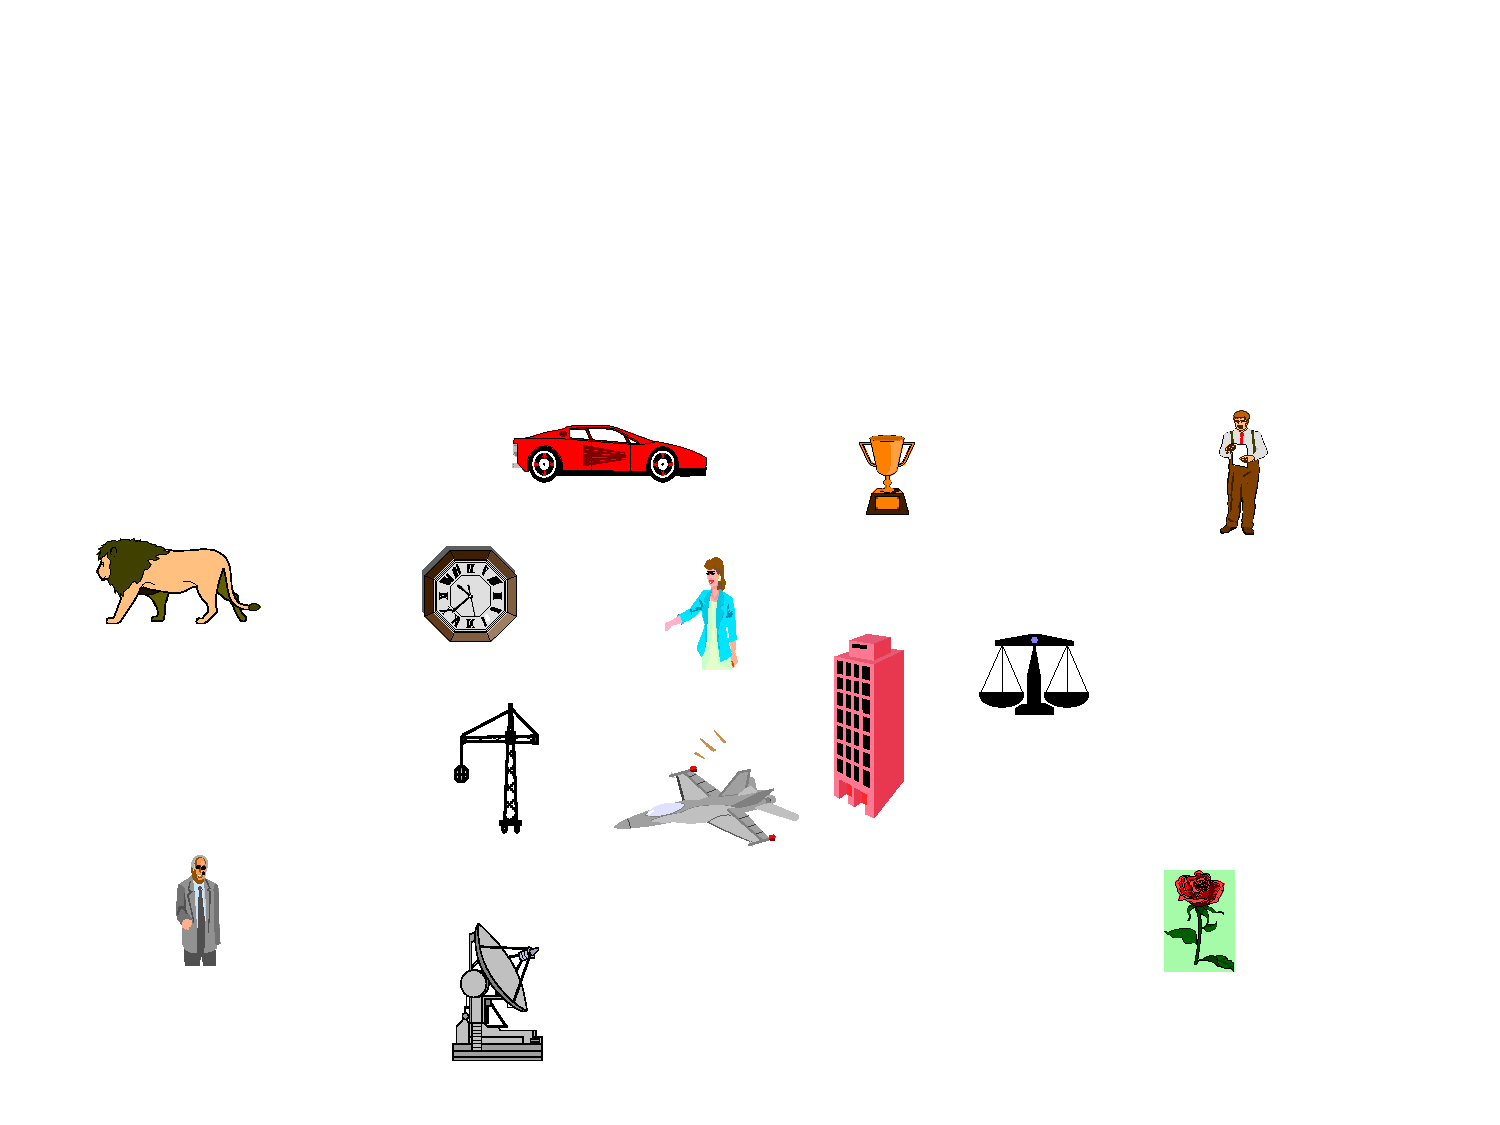
\includegraphics[width=0.8\hsize]{physicalworld.pdf}
    \end{center}
  }

\only<2>{
  (1)被抽象为系统中的对象 \\
    \begin{center}
      \centering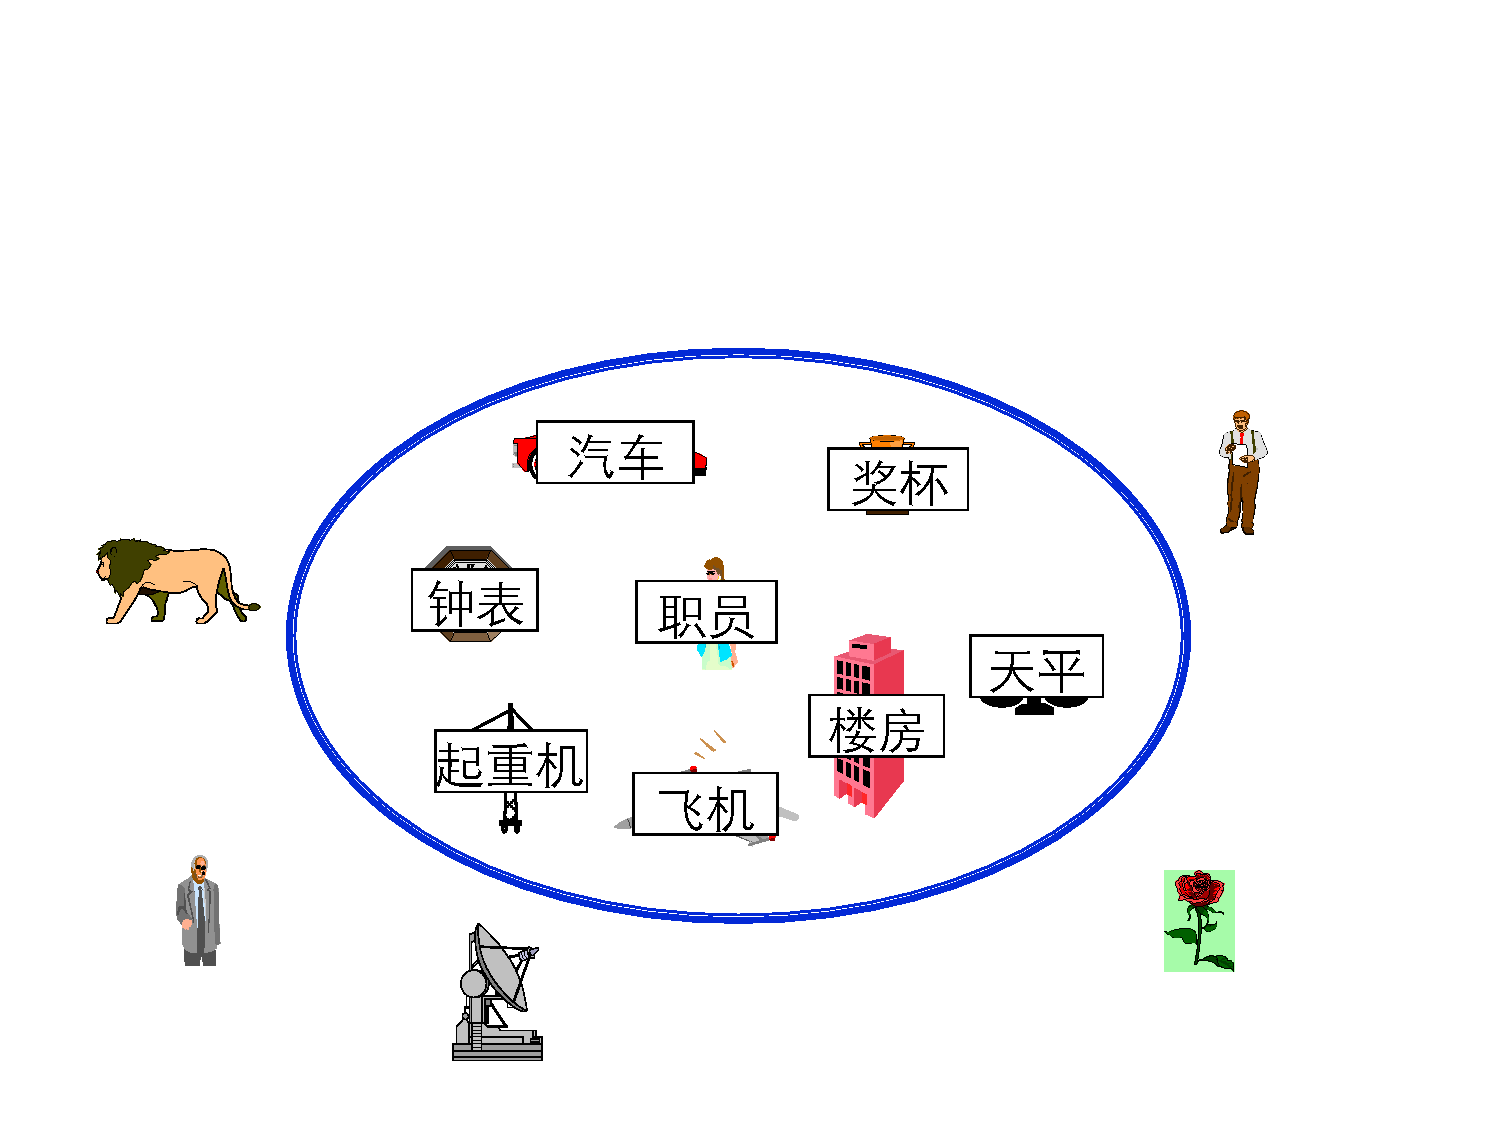
\includegraphics[width=0.8\hsize]{physicalworld-sys.pdf}
    \end{center}
  }

\only<3>{
  (2)只作为系统外部的参与者与系统交互\\
    \begin{center}
      \centering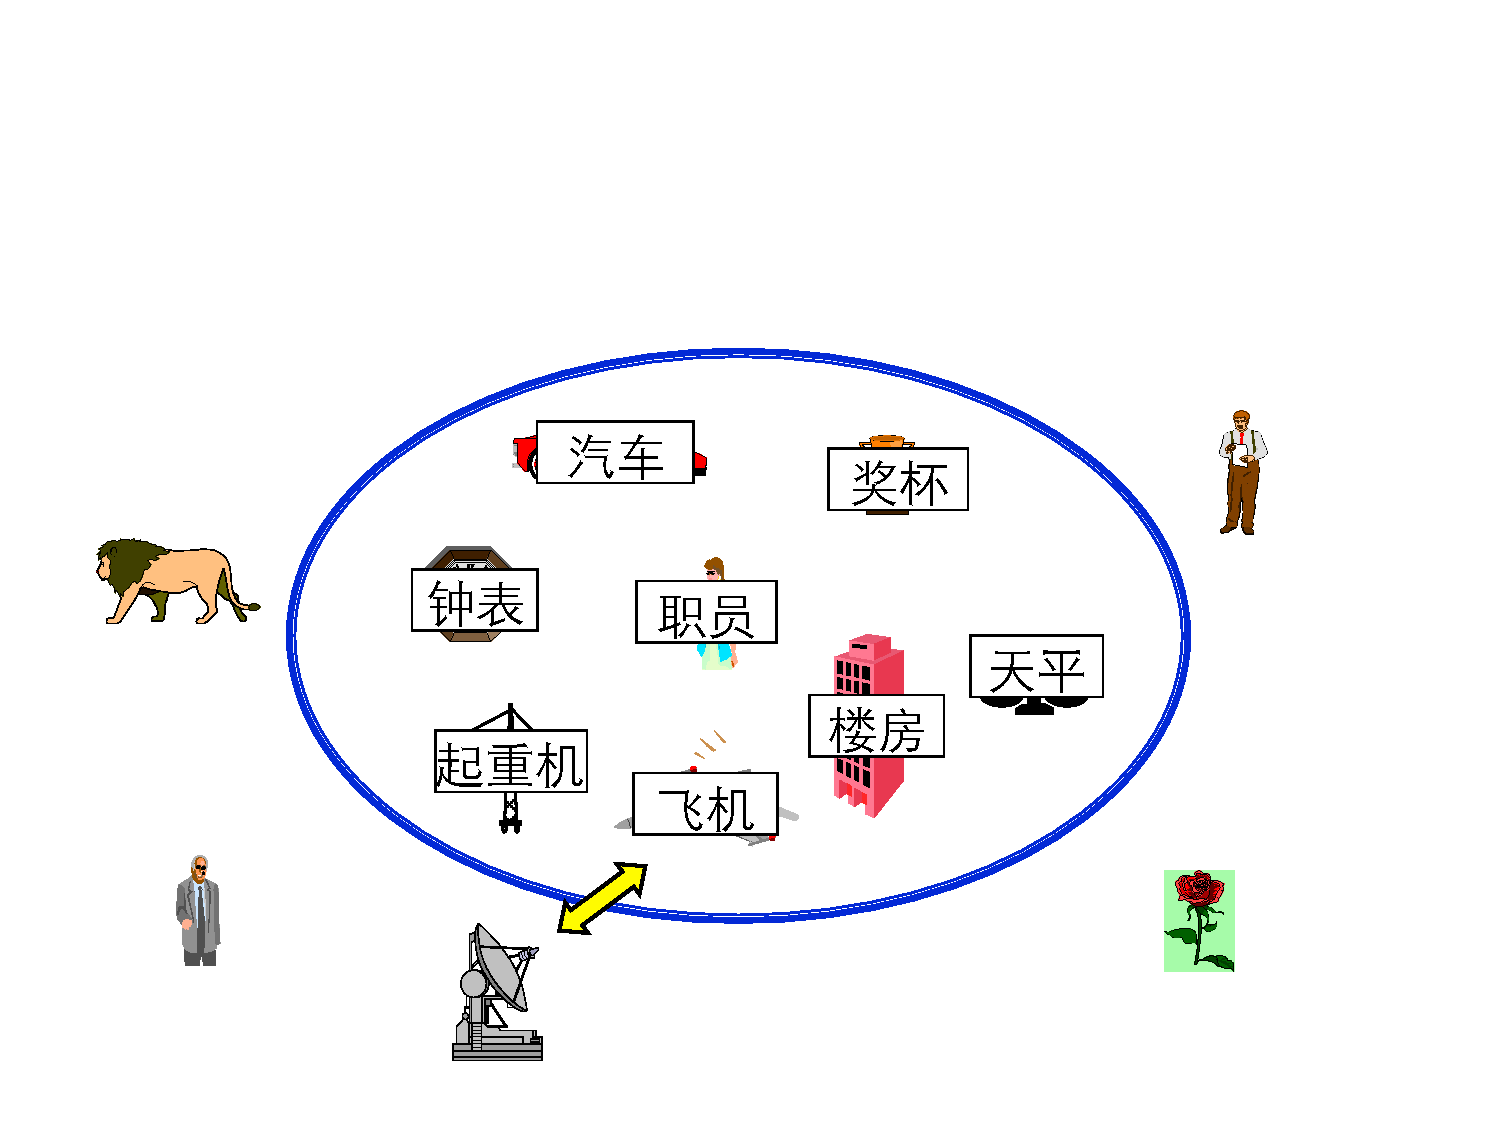
\includegraphics[width=0.8\hsize]{physicalworld-actor.pdf}
    \end{center}
  }

\only<4>{
(3)既是系统中的对象,本身又作为参与者与系统交互 \\
    \begin{center}
      \centering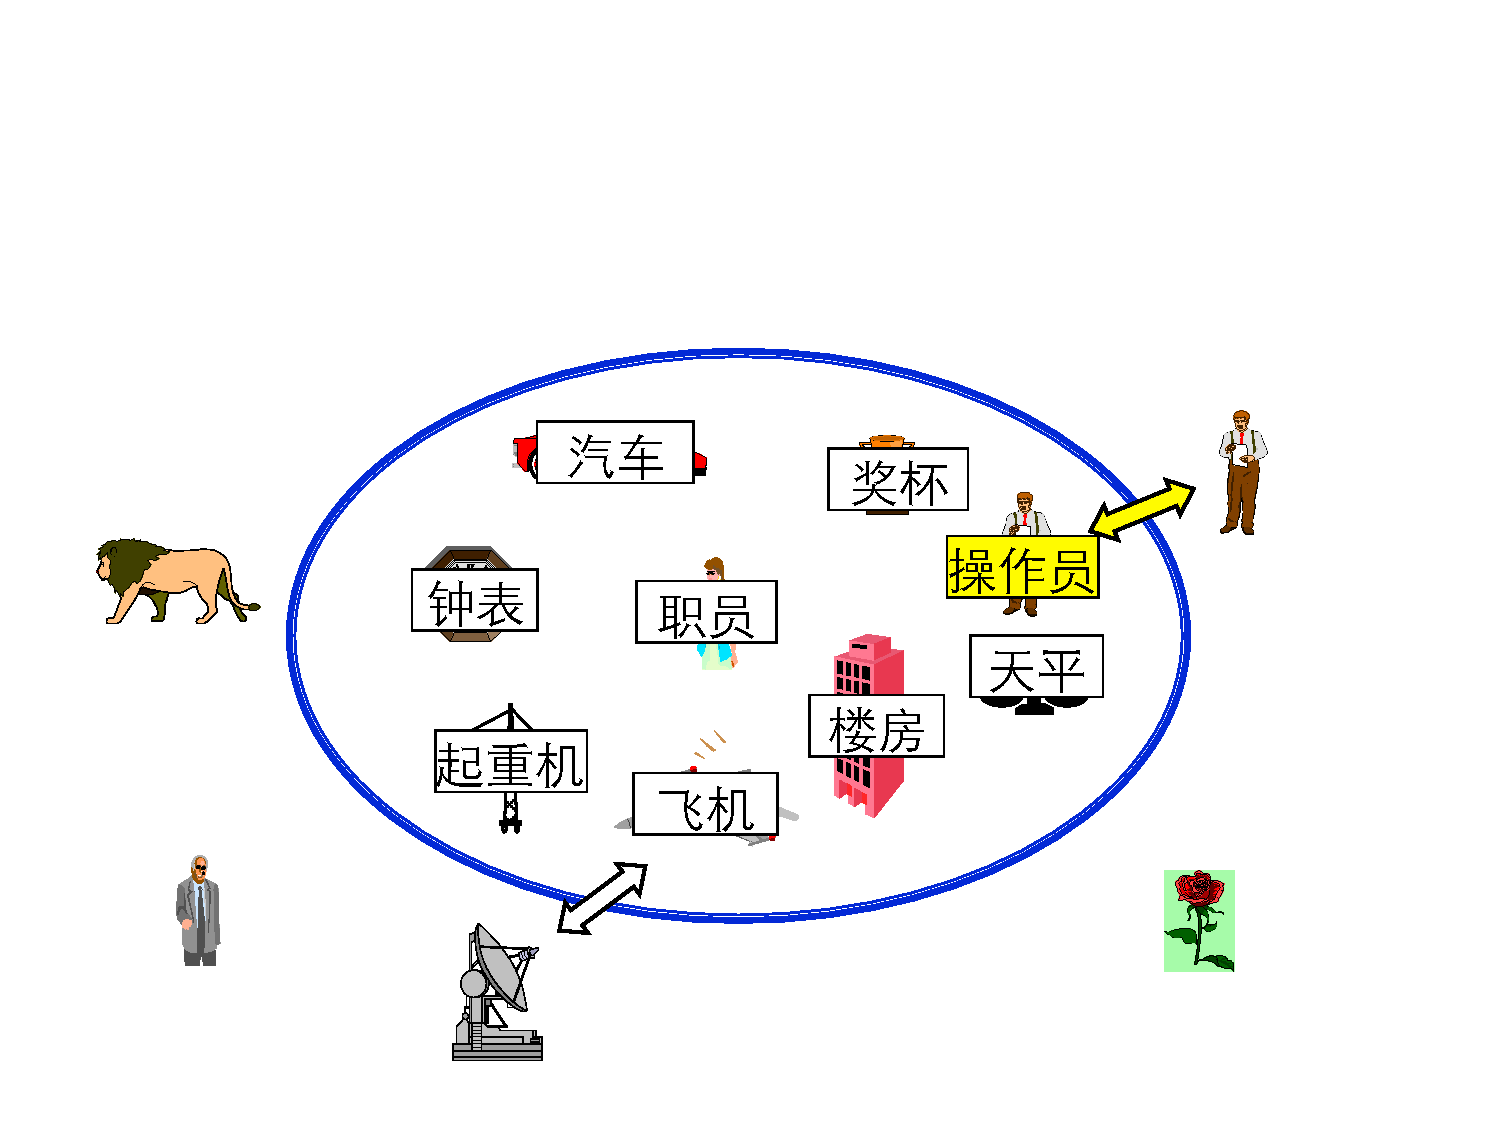
\includegraphics[width=0.8\hsize]{physicalworld-actorop.pdf}
    \end{center}
  }


\only<5>{
  (4)与系统无关 \\
    \begin{center}
      \centering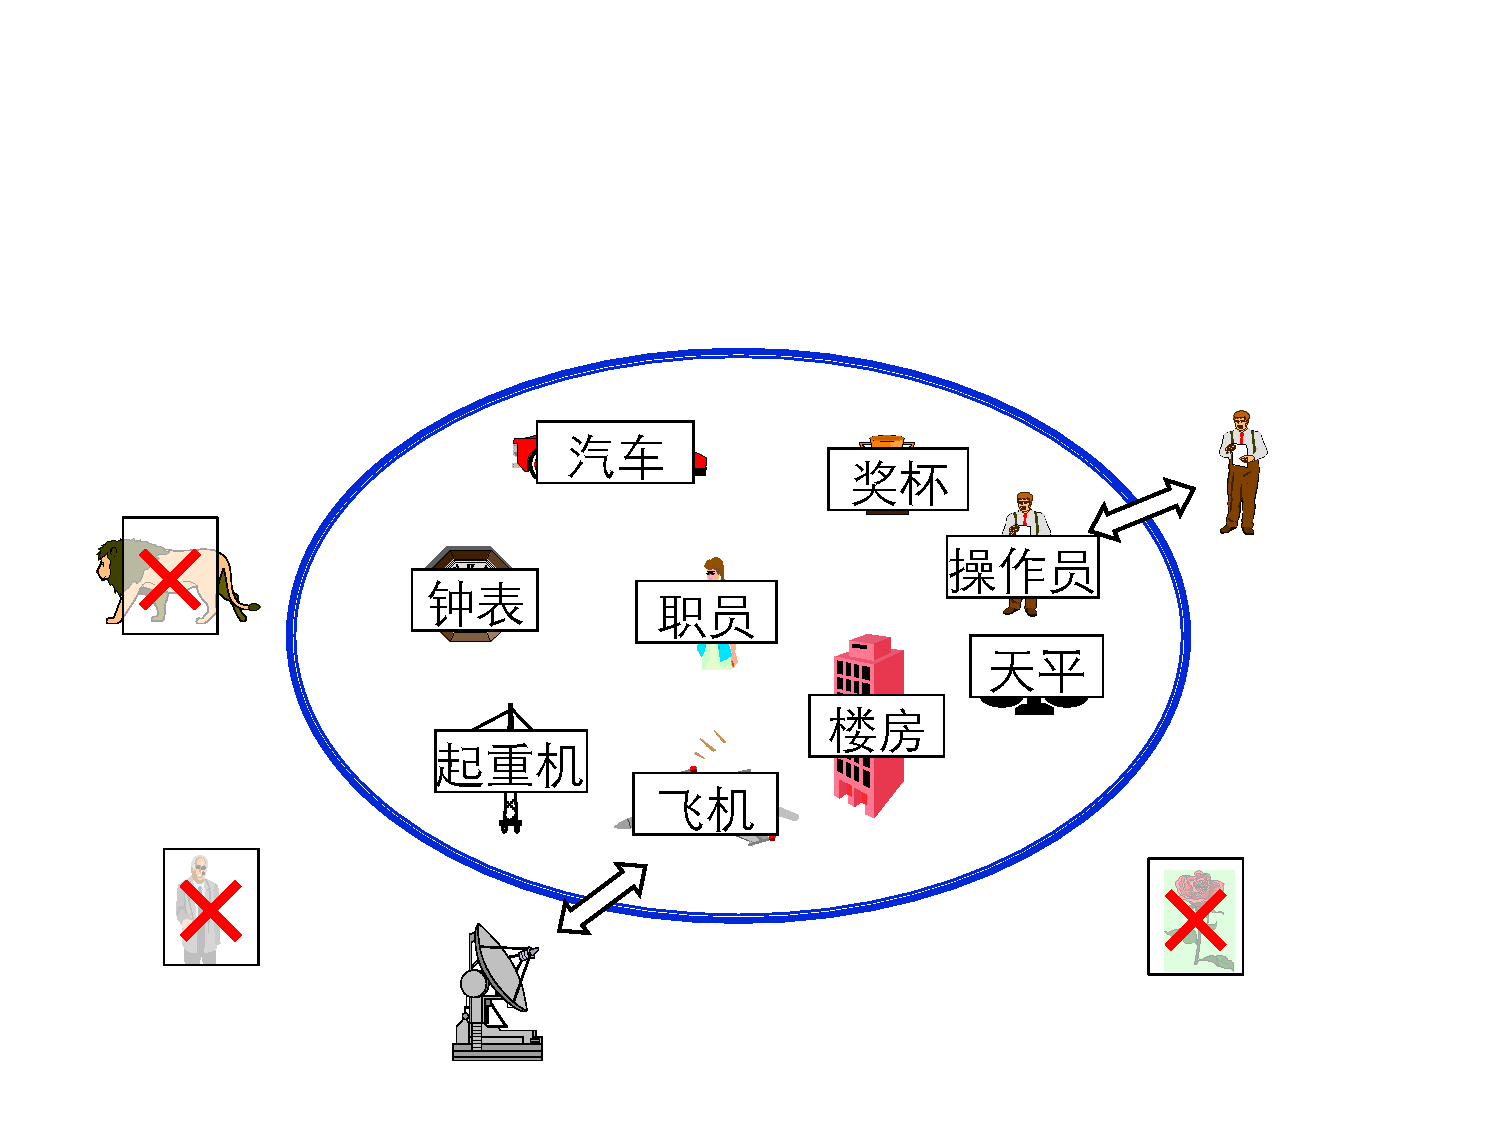
\includegraphics[width=0.8\hsize]{physicalworld-other.pdf}
    \end{center}
  }
  \end{overprint}
\end{frame}

\begin{frame}
  \frametitle{如何发现参与者}
  \begin{columns}[t]
    \column{0.5\hsize}
    \onslide<1->{
    \textbf{人员:}
    \begin{itemize}
      \item 系统的直接使用者 
      \item 直接为系统服务的人员
    \end{itemize}
  }
    \onslide<2->{
    \textbf{外系统:}
    \begin{itemize}
      \item 上级系统
      \item 子系统
      \item 其它系统
    \end{itemize}
  }
    \column{0.5\hsize}
    \onslide<3->{
    \textbf{设备:}
    \begin{itemize}
      \item 与系统直接相联的设备
        \begin{itemize}
          \item 为系统提供信息
          \item 在系统控制下运行
        \end{itemize}
      \item<4-> \alt<4> {\color{black} 不与系统相连的设备} 
        {\color{red} \sout{\mbox{不与系统相连的设备}}}
      \item<6-7> \alt<6> {\color{black} 计算机设备} 
        {\color{red} \sout{\mbox{计算机设备}}}
    \end{itemize}
  }
  \end{columns}
\end{frame}

\begin{frame}
    \frametitle{关于参与者与涉众}
    \begin{itemize}
        \item 涉众是系统的利益相关方
        \item 参与者是系统的主动交互方, 处于边界之外, 获得系统的服务
        \item 涉众不一定直接和系统交互
        \item 参与者常常是因为要满足涉众的目标, 关联涉众的利益而存在
        \item 参与者的职责通常可用角色(Role)表示
        \item 参与者可以是系统的用户
    \end{itemize}
\end{frame}

\subsection{用况}

\begin{frame}
  \frametitle{用况(use case)}
  \begin{block}{《对象技术词典》}
    \begin{enumerate}
      \item 对一个系统或一个应用的一种单一的使用方式所进行的描述
      \item 关于单个参与者在与系统的对话中所执行的处理的行为陈述序列
  \end{enumerate}
  \end{block}
  \begin{block}{ UML }
      对系统在与它的参与者交互时所能执行的一组动作序列(包括其变体)的描
      述
    \end{block}

\end{frame}

\begin{frame}
  \frametitle{用况:本书的定义}
  \begin{definition}
  \textbf{用况}是对参与者使用系统的一项功能时所进行的交互过程的描述,其中包含由双方
交替执行的一系列动作
\end{definition}
\begin{itemize}
  \item 一个用况只描述参与者对\alert{单独一项}系统功能的使用情况
  \item 通常是平铺直叙的\alert{文字}描述,UML也允许其他描述方式
  \item 陈述参与者和系统在交互过程中\alert{双方}所做的事
  \item 所描述的交互既可能由\alert{参与者发起}也可能由\alert{系统发起}
  \item 描述彼此为对方\alert{直接地}做什么事,不描述怎么做
  \item 描述应力求准确,允许概括,但\alert{不要把双方的行为混在一起}
  \item 一个用况可以由\alert{多种参与者}分别参与或共同参与
\end{itemize}
\end{frame}


\begin{frame}
  \frametitle{内容与书写格式}
    \begin{itemize}
      \item 名称
      \item 行为陈述(分左右栏)
      \item 调用语句
      \item 控制语句
      \item 括号或标号
    \end{itemize}
\end{frame}


{
\defverbatim[colored]{\verbcase}{%
   \renewcommand{\baselinestretch}{1.1}
\begin{Verbatim}[commandchars=\\\^\$, fontsize=\small, label=示例]
\textbf^收款$

输入开始本次收款的命令;
        \textblue^作好收款准备,应收款总数置为0,输出提示信息;$
for  顾客选购的每种商品 do
  输入商品编号;
  if  此种商品多于一件 then
    输入商品数量
  end if;
        \textblue^检索商品名称及单价;货架商品数减去售出数;$
        \textblue^if  货架商品数低于下限 then$
             \textblue^call 通知上货$
        \textblue^end if;$
        \textblue^计算本种商品总价并打印编号、名称、数量、单价、总价;$
        \textblue^总价累加到应收款总数;$
end for;
        \textblue^打印应收款总数;$
输入顾客付款数;
        \textblue^计算应找回款数,打印付款数及找回款,计入账册。$
\end{Verbatim}
}

\begin{frame}[plain]
\verbcase
\end{frame}
}

\begin{frame}
  \frametitle{如何定义用况: 针对单个用况的描述策略}
把自己当作参与者,与设想中的系统进行交互。考虑:
\begin{itemize}
  \item 交互的目的是什么?
  \item 需要向系统输入什么信息?
  \item 希望由系统进行什么处理并从它得到何种结果?
\end{itemize}

把上述交互过程描述出来 
\end{frame}

\begin{frame}
  \frametitle{如何定义用况: 定义系统中所有的用况}
  \begin{enumerate}
\item 全面地了解和收集用户所要求的各项系统功能,找出所有的参与者,了解与
各项功能相关的业务流程
\item 把用户提出的功能组织成适当的单位,每一项功能完成一项完整而相对独立
的工作
\item 穷举每一类参与者所使用的每一项系统功能,定义相应的用况
\item 检查用户对系统的各项功能需求是否都通过相应的用况做了描述
\end{enumerate}
\end{frame}

\begin{frame}
  \frametitle{用况图}
  模型元素:参与者、用况、延伸、包含、泛化 \\[2ex]
    %\begin{center}
      %\centering\includegraphics[width=0.8\hsize]{uc-diagram.pdf}
    %\end{center}
\scalebox{0.9}{
\begin{tikzpicture}
\tikzumlset{fill usecase=white}

\begin{umlsystem}[x=3]{系统}
\umlusecase{use case1}
\umlusecase[y=-2]{use case2}
\umlusecase[y=-4]{use case3}
\umlusecase[x=4, y=-2, fill=orange!40]{use case4}
\umlusecase[x=4]{use case5}
\umlusecase[x=4, y=-4]{use case6}
\end{umlsystem}

\umlactor{user}
\umlactor[y=-3]{subuser}
\umlactor[x=10, y=-1.5]{admin}

\umlinherit{subuser}{user}
\umlassoc{user}{usecase-1}
\umlassoc{subuser}{usecase-2}
\umlassoc{subuser}{usecase-3}
\umlassoc{admin}{usecase-5}
\umlassoc{admin}{usecase-6}
\umlinherit{usecase-2}{usecase-1}
\umlextend{usecase-5}{usecase-4}
\umlinclude[name=incl]{usecase-3}{usecase-4}
\end{tikzpicture}
}

\end{frame}

\begin{frame}
  \frametitle{参与者: actor}
    \begin{minipage}[t]{1.2in}
    %\centering\includegraphics[width=0.8in]{actor-default.pdf}

    \centering \tikz \umlactor[scale=1]{Actor} ;

    缺省
    \end{minipage}%    
    \begin{minipage}[t]{1.5in}
    %\centering\includegraphics[width=1.2in]{actor-rectangle.pdf}
    \centering \tikz \node [draw, rectangle, text width=2cm, minimum height=1.5cm, align=center] {<<actor>> \linebreak Customer} ; 

    矩形 
    \end{minipage}%
    \begin{minipage}[t]{1.2in}
    \centering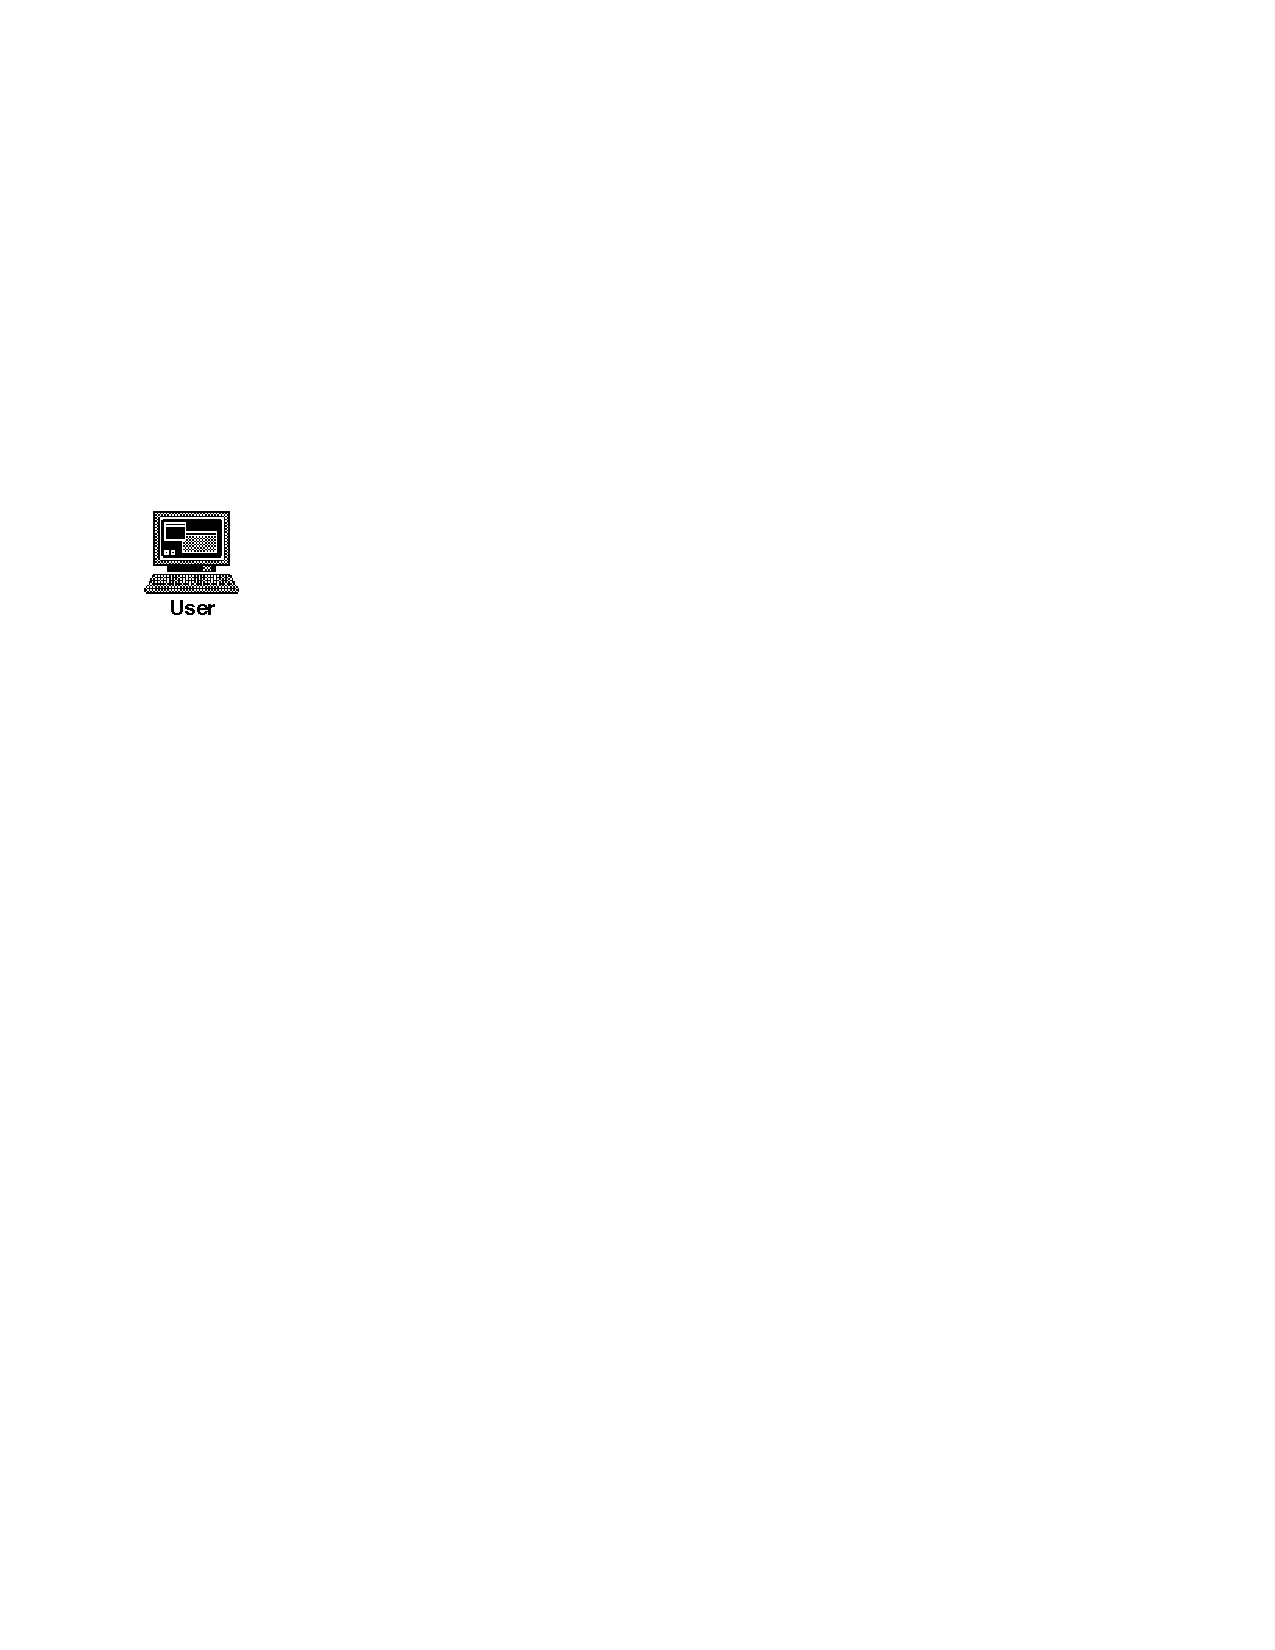
\includegraphics[width=0.8in]{actor-icon.pdf}

    图标
    \end{minipage}
\end{frame}

\begin{frame}
  \frametitle{用况: use case}

  %\begin{columns}[t]
    %\column{0.4\hsize}
    %\begin{center}
      %\centering\includegraphics[height=1.5cm]{uc-default.pdf}
    %\end{center}
%\vfill
    %\begin{center}
      %\centering\includegraphics[height=2cm]{uc-below.pdf}
    %\end{center}
    %\column{0.6\hsize}
    %\begin{center}
      %\centering\includegraphics[height=2cm]{uc-ext.pdf}
    %\end{center}
%\vfill
    %\begin{center}
      %\centering\includegraphics[height=1.2cm]{uc-rectangle.pdf}
    %\end{center}
  %\end{columns}

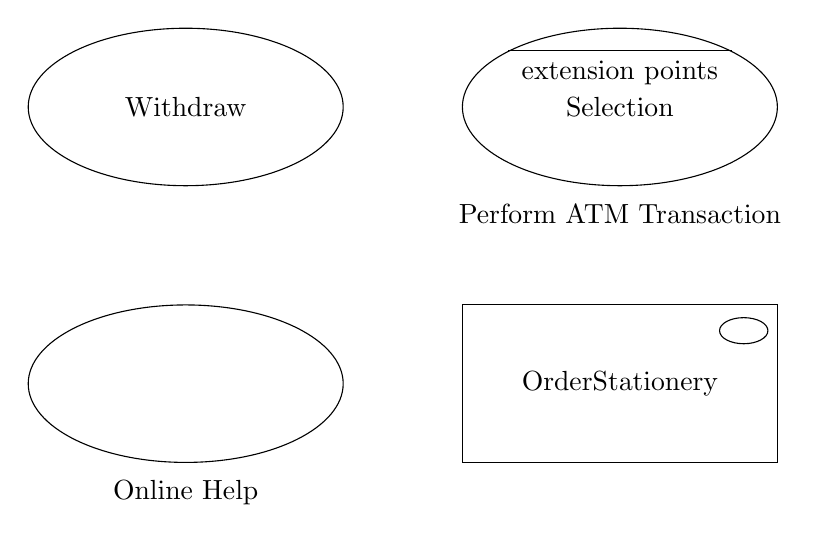
\begin{tikzpicture}
\node [ellipse, draw, minimum width=4cm, minimum height=2cm] (U1) {Withdraw} ;
\node [ellipse, draw, minimum width=4cm, minimum height=2cm, below=1.5cm of U1] (U2) {} ;
\node [below=0.1 of U2] {Online Help} ;

\node [ellipse, draw, minimum width=4cm, minimum height=2cm, right=1.5cm of U1] (U3) {Selection} ;
\path (U3.north east) edge node [below] {extension points} (U3.north west) ;
\node [below=0.1 of U3] {Perform ATM Transaction} ;

\node [rectangle, draw, minimum width=4cm, minimum height=2cm, right=1.5cm of U2] (U4) {OrderStationery} ;
\node [ellipse, draw, text width=0.2cm, below left= 0.3 of U4.north east] {} ;
\end{tikzpicture}

\end{frame}

\begin{frame}
\frametitle{延伸与包含}

\only<1> {
      \begin{block}{包含}
        一个用况中定义的行为\alert{\textbf{包含}}了另一个用况中定义的行
        为. \\
        基用况、被包含用况
      \end{block}
      \vspace*{3ex}
    %\begin{center}
      %\centering\includegraphics[height=1.5cm]{uc-include.pdf}
    %\end{center}
    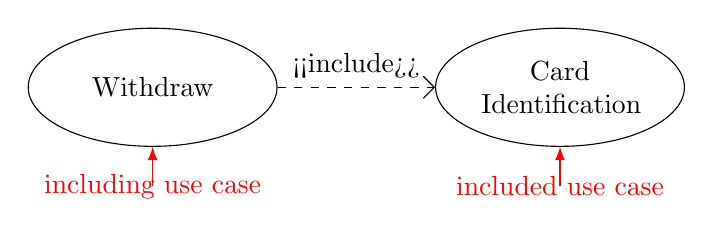
\begin{tikzpicture}
      \renewcommand\baselinestretch{1.0}
      \node [ellipse, draw, text width=2cm, align=center, minimum
      height=1.5cm] (uc1) {Withdraw} ;
      \node [ellipse, draw, right=2 of uc1, minimum height=1.5cm, text width=2cm, align=center] (uc2) {Card
      \\Identification} ;

      \path [-{Straight Barb[length=4pt]}, dashed] (uc1) edge node [above] {<<include>>}  (uc2) ;

      \path [-Latex, red] ([yshift=-0.5cm]uc1.south) edge node [at
      start] {including use case} (uc1.south) ;

      \path [-Latex, red] ([yshift=-0.5cm]uc2.south) edge node [at
      start] {included use case} (uc2.south) ;
    \end{tikzpicture}
  }

  \only<2> {
      \begin{block}{延伸}
        一个用况中定义的行为\alert{\textbf{延伸}}了另一个用况中定义的行
        为. \\
        基用况、延伸用况
      \end{block}
      \vspace*{3ex}
    %\begin{center}
      %\centering\includegraphics[height=1.5cm]{uc-extend.pdf}
    %\end{center}
    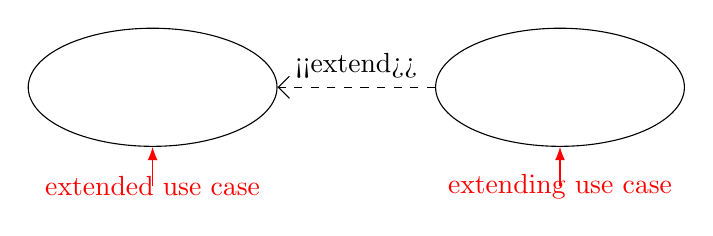
\begin{tikzpicture}
      \node [ellipse, draw, text width=2cm, align=center, minimum
      height=1.5cm] (uc1) {} ;
      \node [ellipse, draw, text width=2cm, minimum height=1.5cm,
      left=2cm of uc1, align=center] (uc2) {} ;
      \path [-{Straight Barb[length=4pt]}, dashed] (uc1) edge node [above] {<<extend>>}  (uc2) ;

      \path [-Latex, red] ([yshift=-0.5cm]uc1.south) edge node [at
      start] {extending use case} (uc1.south) ;

      \path [-Latex, red] ([yshift=-0.5cm]uc2.south) edge node [at
      start] {extended use case} (uc2.south) ;
  \end{tikzpicture}


  }
\end{frame}

\begin{frame}
  \frametitle{延伸和包含的问题}
  \begin{itemize}
    \item 延伸与包含的相似性
    \item 延伸的方向问题
  \end{itemize}
  \begin{block}{建议}
    在难以确定用包含关系还是延伸关系时,不妨选择包含关系
\end{block}
\end{frame}

\begin{frame}
  \frametitle{``条件''和``延伸点''的问题: 内部细节 vs 之间关系}
    %\begin{center}
      %\centering\includegraphics[height=3cm]{uc-extensionpoint.pdf}
    %\end{center}

  \scalebox{0.7}{
  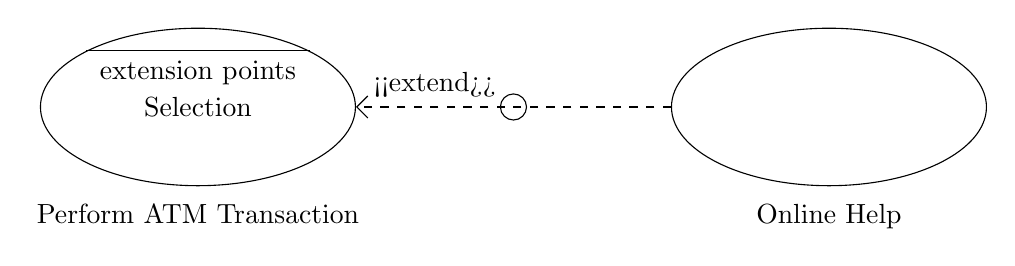
\begin{tikzpicture}
    \node [ellipse, draw, minimum width=4cm, minimum height=2cm] (U2) {} ;
    \node [below=0.1 of U2] {Online Help} ;

    \node [ellipse, draw, minimum width=4cm, minimum height=2cm, left=4cm of U2] (U1) {Selection} ;
    \path (U1.north east) edge node [below] {extension points} (U1.north west) ;
    \node [below=0.1 of U1] {Perform ATM Transaction} ;

    \path [-{Straight Barb[length=4pt]}, dashed] (U2) edge node [near end,  above] {<<extend>>}
    node [circle, draw, solid] (Mid) {} (U1) ;

    \umlnote[x=-2, y=2.5, width=6cm, fill=white] {Mid} {Condition:{customer selected HELP \\} 
  extension point:Selection}

  \end{tikzpicture}
}

  \begin{block}{建议}
    加强用况内部过程的描述,在基用况的描述中清楚表示它对其他用况的调用,
    不要在用况图中过多表现用况内部结构细节
\end{block}
\end{frame}

\begin{frame}
  \frametitle{用况间的泛化关系问题: 语义模糊}
    %\begin{center}
      %\centering\includegraphics[height=3cm]{uc-generalization.pdf}
    %\end{center}

  \noindent\begin{tikzpicture}
    \tikzumlset{fill usecase=white}
    \renewcommand\baselinestretch{1.0}
    \umlusecase[name=uc1]{TransferFunds}
    \umlusecase[x=-4, name=uc2]{Withdraw}
    \umlusecase[x=4, name=uc3]{DepositFunds}
    \umlusecase[y=2, width=2.5cm, name=uc4]{Perform ATM Transaction}
    \umlinherit{uc1}{uc4}
    \umlinherit{uc2}{uc4}
    \umlinherit{uc3}{uc4}
  \end{tikzpicture}

  \vspace*{2ex}

  \begin{block}{建议}
    不要通过泛化来定义用况的行为,尝试采用包含关系准确描述基用况和被包含
    用况之间的行为
\end{block}
\end{frame}

\begin{frame}
  \frametitle{系统、主题及其边界的表示法问题}
    %\begin{center}
      %\centering\includegraphics[height=4.8cm]{uc-atm.pdf}
    %\end{center}

  \noindent\scalebox{0.9}{
  \begin{tikzpicture}
  \tikzumlset{fill usecase=white}

  \begin{umlsystem}[x=5]{ATMSystem}
    \umlusecase[name=uc1]{Withdraw}
  \umlusecase[y=-1, name=uc2]{Transfer Funds}
  \umlusecase[y=-2, name=uc3]{Deposit Money}
  \umlusecase[y=-3, name=uc4]{Register ATM at Bank}
  \umlusecase[y=-4, name=uc5]{Read Log}
  \end{umlsystem}

  \umlactor[y=0]{Customer}
  \umlactor[y=-3]{Administrator}
  \umlactor[x=9.5, y=-3]{Bank}

  \umlinherit{Administrator}{Customer}
  \umlassoc[arg1=1, arg2=0..1]{Customer}{uc1}
  \umlassoc[arg1=1, arg2=0..1]{Customer}{uc2}
  \umlassoc[mult1=1, mult2=0..1]{Customer}{uc3}
  \umlassoc[arg1=1, arg2=0..1]{Administrator}{uc4}
  \umlassoc[mult1=1, mult2=0..1]{Administrator}{uc5}
  \umlassoc[arg1=1, arg2=0..*]{Bank}{uc4}
  \umlassoc[mult1=1, mult2=0..*]{Bank}{uc3}
  \end{tikzpicture}
}

\noindent  建议: 最重要的是正确描述需求,边框是不是系统边界不必深究
\end{frame}

\begin{frame}
  \frametitle{两个(或多个)参与者共享一个用况}
    %\begin{center}
      %\centering\includegraphics[width=0.7\hsize]{uc-share.pdf}
    %\end{center}
  \begin{tikzpicture}
  \tikzumlset{fill usecase=white}

  \begin{umlsystem}[x=4]{}
    \umlusecase[name=uc1]{系统维护}
    \umlusecase[y=-2, name=uc2]{登录}
  \end{umlsystem}

  \umlactor[y=0]{系统管理员}
  \umlactor[y=-2]{普通用户}

  \umlassoc{系统管理员} {uc1}
  \umlassoc{系统管理员} {uc2}
  \umlassoc{普通用户} {uc2}

\end{tikzpicture}

  \end{frame}

  \begin{frame}
    \frametitle{一个用况的执行需要多个参与者}
  %  \begin{center}
  %    \centering\includegraphics[width=0.9\hsize]{uc-collab.pdf}
  %  \end{center}
  \begin{tikzpicture}
  \tikzumlset{fill usecase=white}

  \begin{umlsystem}[x=4]{}
    \umlusecase[name=uc1]{网上购物}
  \end{umlsystem}

  \umlactor{客户}
  \umlactor[x=8]{供货商}

  \umlassoc{客户} {uc1}
  \umlassoc{供货商} {uc1}
  \end{tikzpicture}

  \end{frame}

  \begin{frame}
    \frametitle{用况及其状态机}
    %\begin{center}
      %\centering\includegraphics[width=0.6\hsize]{uc-statemachine.pdf}
    %\end{center}

    \centering\scalebox{0.8}{
    \begin{tikzpicture}
      \begin{umlstate}[fill=white]{usecase MakeCall}
        \begin{umlstate}[fill=white]{statemachine Call}
        \umlstateinitial[name=Sinit]
        \node [rounded rectangle, draw, inner sep=2pt, below=1.5cm of Sinit.center] (Dialing) {Dialing} ;
        \node [rounded rectangle, draw, inner sep=2pt, below=1.5cm of Dialing.center] (Ringing) {Ringing} ;
        \node [rounded rectangle, draw, inner sep=2pt, below=1.5cm of Ringing.center] (Talking) {Talking} ;
        \umlstatefinal[x=4, y=-5.25, name=Sfinal]

        \umltrans{Sinit}{Dialing}
        \umltrans[arg=lastDigit, pos=0.5]{Dialing}{Ringing}
        \umltrans[arg=answer, pos=0.5]{Ringing}{Talking}
        \umltrans[arg=onHook, pos=0.5]{Talking}{Sfinal}
      \end{umlstate}
      \end{umlstate}
    \end{tikzpicture}
  }
  \end{frame}

  \begin{frame}[label=current]
    \frametitle{用况与包}
    \begin{center}
      \centering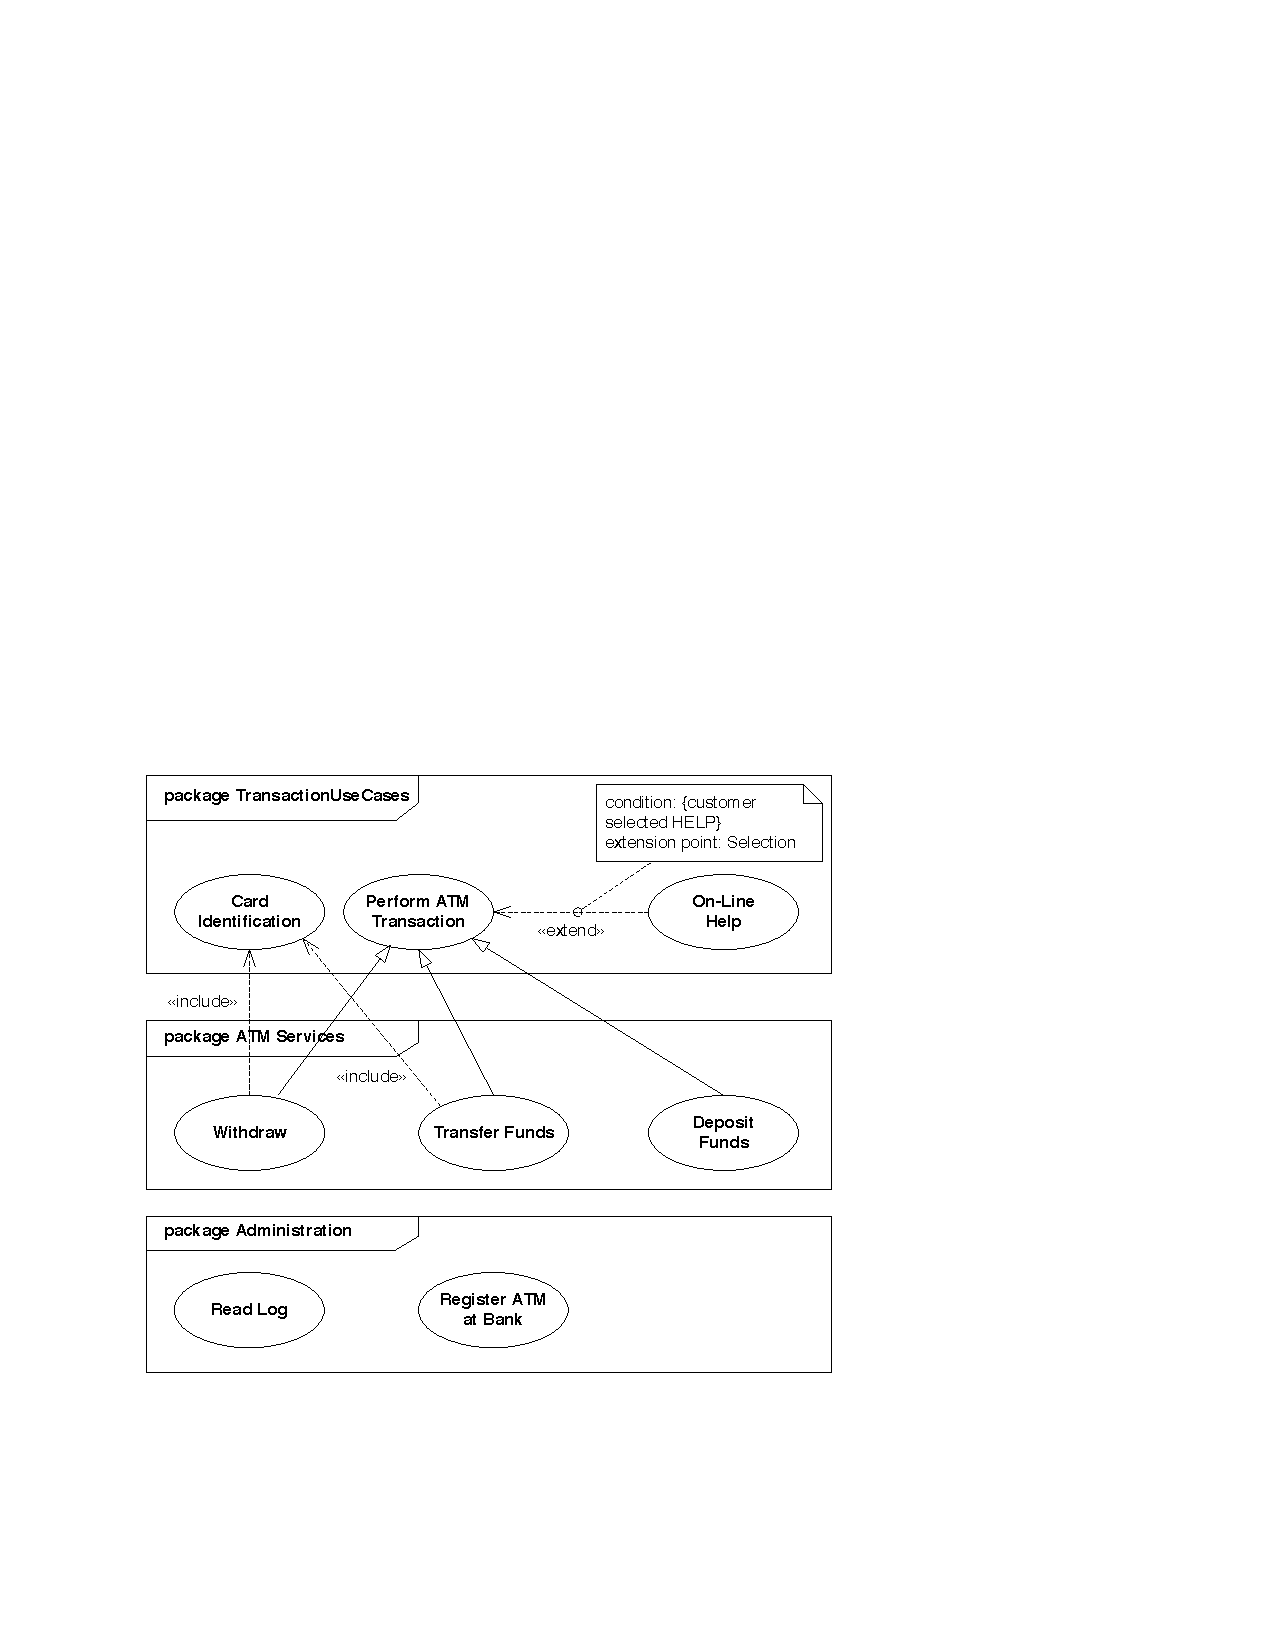
\includegraphics[width=0.75\hsize]{uc-package.pdf}
    \end{center}
  \end{frame}



  \begin{frame}
    \frametitle{用况图的开发过程}
    \begin{itemize}
      \item 确定系统边界
      \item 发现参与者 
      \item 定义用况 
      \item 建立用况之间的关系 
      \item 确定参与者和用况之间的关系 
      \item 绘制用况图 
    \end{itemize}
  \end{frame}

  \begin{frame}
    \frametitle{使用用况图的建议小结}
    \begin{itemize}
      \item 最重要的工作是对用况的描述
      \item 不要过分深入地描述系统内部的行为细节 
      \item 运用最主要概念,加强用况内容的描述
        \begin{itemize}
          \item 不要陷入延伸与包含、延伸点、泛化等问题的争论和辨别
    \end{itemize}
      \item 了解用况的局限性——主要作用是描述功能需求
        \begin{itemize}
          \item 非功能需求?
        \end{itemize}
    \end{itemize}
  \end{frame}

  \section{建立对象类}

  \subsection{概念与表示法}

  \begin{frame}
    \frametitle{概念}
    \begin{block}{对象(object)}
        是系统中用来描述客观事物的一个实体,它是构成系统的
        一个基本单位,由一组属性和施加于这组属性的一组操作构成
    \end{block}
    \begin{block}{类(class)}
      是具有相同属性和操作的一组对象的集合,它为属于该类的全
      部对象提供了统一的抽象描述,它由一个类名、一组属性和一组操作构成。 

    \end{block}
  \end{frame}

  \begin{frame}
    \frametitle{类与实例}
    \begin{itemize}
      \item 类和对象的关系——集合与成员,对象是类的实例
      \item 在一般-特殊结构中,特殊类的对象实例在逻辑上也都是其一般类的
        对象实例
      \item 不直接创建对象实例的类称为\alert{抽象类}(abstract class) 
  \end{itemize}
    %\begin{center}
      %\centering\includegraphics[width=0.4\hsize]{c-student.pdf}
    %\end{center}

  \centering\begin{tikzpicture}
    \tikzumlset{fill class=white}
    \umlsimpleclass[type=abstract]{学生}
    \umlsimpleclass[x=-1, y=-2] {本科生}
    \umlsimpleclass[x=1, y=-2] {研究生}
    \umlinherit[geometry=|-|]{本科生}{学生}
    \umlinherit[geometry=|-|]{研究生}{学生}
  \end{tikzpicture}
  \end{frame}

  \begin{frame}
    \frametitle{主动对象与被动对象}
    \begin{block}{主动对象(active object)}
      至少有一个操作不需要接收消息就能主动执行的对象,
    用于描述具有主动行为的事物

    主动对象的类叫做\alert{主动类}(active class)
  \end{block}

  \begin{block}{被动对象(passive object)}
   每个操作都必须在消息的驱动下才能执行的对象
 \end{block}

  \end{frame}

  \begin{frame}
    \frametitle{类的语义 ~~ 1 }

    一个类代表由它的全部对象实例所构成的群体
    \begin{example}
      \begin{itemize}
        \item “公司里有管理人员、技术人员和市场人员”
        \item “马路上汽车很多” 
      \end{itemize}
    \end{example}

    在OO模型中,每个类都是由它的全部对象实例所构成的集合,
    类代表了它的全部对象实例
  \end{frame}

  \begin{frame}
    \frametitle{类的语义 ~~ 2 }
    一个类代表属于该类的任意一个对象实例,
    从大量的个体中抽象出一个概念,运用该概念时可以代表其中的任何一
    个个体
    \begin{example}
      “学生有一个学号,属于一个班级,要上课” 
    \end{example}
    OO系统模型中的\alert{类}可以代表它的任何一个对象实例
    \begin{example}
    汽车与发动机之间的聚合关系,表示任何一辆汽车都有一台发动机,任何一台
    发动机都可以装在0—1辆汽车上
  \end{example}

  \end{frame}

  \begin{frame}
    \frametitle{在类的抽象层次建模}
    \begin{itemize}
      \item 充分性:模型中一个类描述了它的全部对象实例
      \item 必要性:个别对象实例不能代表其他对象实例
      \item 符合人类的思维方式:在概念层次上表达描述事物规律
      \item 与OOPL保持良好的对应
      \item 避免建模概念复杂化 
      \item 消除抽象层次的混乱
\end{itemize}
  \end{frame}

  \begin{frame}
    \frametitle{如何运用类和对象的概念}
    
    \begin{block}{归纳}
      从对象出发认识问题域,将问题域中的事物抽象为对象

      将具有共同特征的对象抽象为类,用类以及它们之间的关系构成整个系统模型
    \end{block}
    \begin{block}{演绎}
      在模型中用类表示属于该类的任何对象,在类的规约中说明这个类将创建那些对象实例

      在程序中用类定义它的全部对象,编程时静态声明类,运行时动态创建类的对象

    \end{block}
  \end{frame}

  \begin{frame}
    \frametitle{表示法}
    %\begin{center}
      %\centering\includegraphics[width=0.6\hsize]{c-notation.pdf}
    %\end{center}
    \centering\begin{tikzpicture}
      \tikzumlset{fill class=white}
      \umlclass[x=4]{Class A}{属性名:类型名 \\ \ldots\ldots}{操作名() \\
      \ldots\ldots}
      \umlsimpleclass{Class B}

      \node at (0, -2.5) {压缩方式} ;
      \node at (4, -2.5) {展开方式} ;
    \end{tikzpicture}
  \end{frame}

  \begin{frame}
    \frametitle{主动类表示法}
      %\includegraphics[width=0.45\hsize]{c-active.pdf}%
      %\hfill\includegraphics[width=0.3\hsize]{c-active-uml2.pdf}
\begin{tikzpicture}
  \tikzumlset{fill class=white}
  \umlemptyclass[type=active]{Class A}
  \umlemptyclass[x=2.5, type=主动]{Class B}
  \umlemptyclass[x=6]{Class C}

  \umlnote [x=1.5, y=2.5, width=4cm] {Class A} {用衍型(stereotype) 表示}

  \draw (Class C.north west) -- ++(-0.1cm, 0) |- (Class C.south west) ;
  \draw (Class C.north east) -- ++(+0.1cm, 0) |- (Class C.south east) ;


  \node at (1.5, -2) {主动类} ;
  \node at (6, -2) {UML2主动类} ;
\end{tikzpicture}

  \end{frame}

  \begin{frame}
    \frametitle{UML的对象表示法}
    %\begin{center}
      %\centering\includegraphics[width=0.7\hsize]{o-notation.pdf}
    %\end{center}
\noindent\begin{tikzpicture}[every text node part/.style={align=center}]
      \node[rectangle split, rectangle split parts=3, draw, text width=2.75cm]
        (O1) { \uline{小王:学生}
          \nodepart{two}
          age:int \\
          name:String
          \nodepart{three}
          getAge():int \\
          getName():String};
      \node[rectangle split, rectangle split parts=3, draw, text width=2.75cm, right = of O1]
        (O2) { \uline{:学生}
          \nodepart{two}
          age:int \\
          name:String
          \nodepart{three}
          getAge():int \\
          getName():String};
       \node[rectangle split, rectangle split parts=3, draw, text width=2.75cm, right = of O2]
        (O3) { :类名
          \nodepart{two}
          属性名:类型 \\
          ......
          \nodepart{three}
          方法名():类型 \\
          ......};

      \node [below = 0.2 of O2] {细节方式} ;
 
      \node[rectangle, draw, text width=2.75cm, below = 1.5 of O1] (O4) {\uline{对象名:类名}} ;
      \node[rectangle, draw, text width=2.75cm, right = of O4] (O5)  {\uline{:类名}} ;
      \node[rectangle, draw, text width=2.75cm, right = of O5] {:类名} ;
      \node [below = 0.2 of O5] {压缩方式} ;
    \end{tikzpicture}
  \end{frame}

  \subsection{发现对象}

  \begin{frame}
    \frametitle{研究问题域 ~~ 1} 
    \begin{itemize}
      \item 亲临现场深入调查研究

    直接观察并向用户及相关的业务人员进行调查和交流,考察问题域中各种各样
    的事物、它们的特征及相互关系 
  \item  听取问题域专家的见解

    领域专家——包括技术人员、管理者、老职员和富有经验的工人等

\end{itemize}
  \end{frame}

  \begin{frame}
    \frametitle{研究问题域 ~~ 2}
    \begin{itemize}
  \item  阅读相关材料

    阅读各种与问题域有关的材料,学习相关行业和领域的基本知识
  \item  借鉴以往的系统

    查阅以往在该问题域中开发过的同类系统的分析文档 ,吸取经验,发现可以
    复用的类
\end{itemize}
\end{frame}

\begin{frame}[shrink=10]
  \frametitle{围绕系统责任对问题域进行正确抽象}
  \begin{itemize}
    \item<1-> 忽略与系统责任无关的事物
  \begin{example}
    学校的教师、学生、教务员,  \alt<1>{警卫} {\color{gray} \sout{\mbox{警
    卫}}}
\end{example}

  \item<3-> 忽略与系统责任无关的事物特征
  \begin{example}
    教师的专业、职称,  \alt<3>{身高、体重}{\color{gray} \sout{\mbox{身高、
    体重}}}
\end{example}

  \item<5-> 正确地提炼对象  
  \begin{example}
    图书馆管理系统中以\alert{一本书}作为一个对象实例

    书店管理系统中以\alert{一种书}作为一个对象实例
\end{example}
\end{itemize}
\end{frame}

\begin{frame}
  \frametitle{策略与启发: 考察问题域}
    %\begin{center}
      %\centering\includegraphics[width=0.8\hsize]{problemdomain.pdf}
    %\end{center}
    \centering\begin{tikzpicture}[every node/.style={rectangle, draw, rounded
      corners, text width=2cm, align=center, inner sep=4pt}]
      \node (O1) {人员} ;
      \node [right = of O1] (O2) {组织} ;
      \node [right = of O2] (O3) {物品} ;
      \node [below = of O1] (O4) {设备} ;
      \node [right = of O4] (O5) {抽象事物} ;
      \node [right = of O5] (O6) {事件} ;
      \node [below = of O4] (O7) {文件} ;
      \node [right = of O7] (O8) {结构} ;
      \node [right = of O8] (O9) {其他} ;
    \end{tikzpicture}
\end{frame}

\begin{frame}
  \frametitle{考察问题域: 人员、组织、物品}
  \begin{itemize}
    \item 人员:由系统管理或使用其信息,或者在系统中呈现某些行为的各类人员
    \item 组织:由系统管理或使用其信息,或者在系统中呈现某些行为的各类组
      织
    \item 物品:由系统进行管理的各种物品
  \end{itemize}
    %\begin{center}
    %  \centering\includegraphics[width=0.5\hsize]{problemdomain.pdf}
    %\end{center}
    \centering\begin{tikzpicture}[every node/.style={rectangle, draw, rounded
      corners, text width=2cm, align=center, inner sep=4pt}]
      \node [red] (O1) {人员} ;
      \node [right = of O1, red] (O2) {组织} ;
      \node [right = of O2, red] (O3) {物品} ;
      \node [below = 0.5 of O1] (O4) {设备} ;
      \node [right = of O4] (O5) {抽象事物} ;
      \node [right = of O5] (O6) {事件} ;
      \node [below = 0.5 of O4] (O7) {文件} ;
      \node [right = of O7] (O8) {结构} ;
      \node [right = of O8] (O9) {其他} ;
    \end{tikzpicture}
\end{frame}

\begin{frame}
  \frametitle{考察问题域: 设备、抽象事物、事件}
  \begin{itemize}
    \item 设备:由系统进行管理或控制,或者在系统中呈现某些行为的各种设备
    \item 抽象事物:如课程、计划、交易、账户
    \item 事件:需要长期记忆的事件,如银行的取款、存款,保险公司的索赔
      ,车辆管理中的驾驶违章
  \end{itemize}
    %\begin{center}
      %\centering\includegraphics[width=0.5\hsize]{problemdomain.pdf}
    %\end{center}
    \centering\begin{tikzpicture}[every node/.style={rectangle, draw, rounded
      corners, text width=2cm, align=center, inner sep=4pt}]
      \node (O1) {人员} ;
      \node [right = of O1] (O2) {组织} ;
      \node [right = of O2] (O3) {物品} ;
      \node [below = 0.5 of O1, red] (O4) {设备} ;
      \node [right = of O4, red] (O5) {抽象事物} ;
      \node [right = of O5, red] (O6) {事件} ;
      \node [below = 0.5 of O4] (O7) {文件} ;
      \node [right = of O7] (O8) {结构} ;
      \node [right = of O8] (O9) {其他} ;
    \end{tikzpicture}
\end{frame}

\begin{frame}
  \frametitle{考察问题域: 文件、结构、其他}
  \begin{itemize}
    \item 文件:泛指各种表格、档案、证件、票据等文件,如业务报表,人事
      档案,身份证,合同,商品订单等
    \item 结构:从结构得到启发,联想到新的对象
    \item 其他:其他一切有助于发现对象的事物
  \end{itemize}
    %\begin{center}
    %  \centering\includegraphics[width=0.5\hsize]{problemdomain.pdf}
    %\end{center}
    \centering\begin{tikzpicture}[every node/.style={rectangle, draw, rounded
      corners, text width=2cm, align=center, inner sep=4pt}]
      \node (O1) {人员} ;
      \node [right = of O1] (O2) {组织} ;
      \node [right = of O2] (O3) {物品} ;
      \node [below = 0.5 of O1] (O4) {设备} ;
      \node [right = of O4] (O5) {抽象事物} ;
      \node [right = of O5] (O6) {事件} ;
      \node [below = 0.5 of O4, red] (O7) {文件} ;
      \node [right = of O7, red] (O8) {结构} ;
      \node [right = of O8, red] (O9) {其他} ;
    \end{tikzpicture}
\end{frame}


\begin{frame}
  \frametitle{文件对象的几个问题}
  \begin{itemize}
    \item 非基础数据
      \begin{example}
        由有限的基础原始数据生成大量各式表格
      \end{example}
    \item 同一事物的重复描述
      \begin{example}
       身份证件、登记表、户籍档案等对象 vs 人员设备对象 
      \end{example}
    \item 多种事物信息组合
      \begin{example}
        网球场地预定表格:场次、收费、姓名、电话、俱乐部账号
      \end{example}
  \end{itemize}
\end{frame}

\begin{frame}
  \frametitle{策略与启发: 考察系统边界}
  考察在系统边界以外与系统交互的各类参与者

  考虑通过那些对象处理这些参与者的交互 \\[3ex]
    %\begin{center}
      %\centering\includegraphics[width=0.9\hsize]{boundary.pdf}
    %\end{center}
    \centering\begin{tikzpicture}[every node/.style={rectangle, draw, rounded
      corners, text width=2cm, align=center, inner sep=4pt}]
      \node (O1) {人员} ;
      \node [right = of O1] (O2) {设备} ;
      \node [right = of O2] (O3) {外系统} ;
    \end{tikzpicture}
 
\end{frame}

\begin{frame}
  \frametitle{策略与启发: 考察系统责任}
  检查每一项功能需求是否已有相应的对象提供,
  发现遗漏的对象
\end{frame}

\begin{frame}
  \frametitle{审查与筛选: 舍弃无用对象}
  \begin{itemize}
    \item 通过属性判断:
      \begin{itemize}
        \item 是否通过属性记录了某些有用的信息?
  \end{itemize}

\item 通过操作判断:
  \begin{itemize}
    \item 是否通过操作提供了某些有用的功能?
  \end{itemize}
  \end{itemize}
      二者都不是——无用
\end{frame}

\begin{frame}
  \frametitle{审查与筛选: 精简对象}
  重点考察只有1个属性/操作的对象\\[3ex]

    %\begin{center}
      %\centering\includegraphics[width=0.9\hsize]{1attribute.pdf}
    %\end{center}
    \noindent\begin{tikzpicture}
      \tikzumlset{fill class=white}
      \umlemptyclass[width=2cm]{班级}
      \umlclass[x=4, width=3cm]{班主任}{姓名}{}
      \umlassoc[mult1=1, mult2=1]{班级}{班主任}
      \node [single arrow, draw, right=0.2 of 班主任, text width=0.4cm] {} ;
      \umlclass[x=8.5, width=3cm]{班级}{班主任姓名}{}

      \umlemptyclass[y=-3, width=1.8cm]{输出设备}
      \umlclass[y=-3, x=4, width=3cm]{格式转换器}{}{文件格式转换}
      \umldep[stereo=call]{输出设备}{格式转换器}
      \node [single arrow, draw, right=0.2 of 格式转换器, text width=0.4cm] {} ;
      \umlclass[y=-3, x=8.5, width=3cm]{输出设备}{}{文件格式转换}

    \end{tikzpicture}

    %\begin{center}
      %\centering\includegraphics[width=0.9\hsize]{1method.pdf}
    %\end{center}
\end{frame}

\begin{frame}
  \frametitle{审查与筛选: 与实现条件有关的对象}
  与实现条件有关的对象可以推迟到OOD阶段考虑,例如:
  \begin{itemize} 
    \item 图形用户界面(GUI)
    \item 数据管理系统
    \item 硬件
    \item 操作系统有关的对象
  \end{itemize}
\end{frame}

\begin{frame}
  \frametitle{对象分类及审查调整}
  \begin{itemize}
    \item 类的属性或操作不适合该类的全部对象实例, 考虑重新分类
      \begin{itemize}
        \item \textcolor{blue}{例}:“汽车”类的“乘客限量”属性不适合于货车
      \end{itemize}
    \item 属性及操作相同的类, 考虑合并
      \begin{itemize}
        \item \textcolor{blue}{例}:作为商品的“服装”和“计算机”
      \end{itemize}
    \item 属性及操作相似的类, 考虑能否提升出一个一般类
      \begin{itemize}
        \item \textcolor{blue}{例}:“轿车”和“货车”抽象出“汽车”
      \end{itemize}
    \item 同一事物的重复描述, 考虑取消其中一个
      \begin{itemize}
        \item \textcolor{blue}{例}:“工作证”和“职员”
      \end{itemize}
  \end{itemize}
\end{frame}

\begin{frame}
  \frametitle{类的命名}
  \begin{itemize}
    \item 类的名字应适合该类(及其特殊类)的全部对象实例
    \item 反映个体而不是群体
    \item 使用名词或带定语的名词
    \item 避免市井俚语和无意义的符号
    \item 使用问题域通用的词汇
    \item 使用便于交流的语言文字
    \item 可以用本地文字和英文双重命名

  \end{itemize}

\end{frame}


\section{定义对象特征}

\subsection{定义属性}

\begin{frame}
  \frametitle{属性}
  \begin{block} {属性(attribute)}
    是用来描述对象静态特征的一个数据项

    \textbf{实例属性}(instance attribute): 各对象实例各自拥有的属性

    \textbf{类属性}(class attribute): 类的所有对象共同拥有的属性

  \end{block}


  \begin{example}
  对于一个仪表类
  \begin{itemize}
    \item 类属性: 输入电压、功率及各种规定的质量指标
    \item 实例属性: 编号、出厂日期、精度等实际性能参数
  \end{itemize}
\end{example}

\end{frame}

\begin{frame}
  \frametitle{操作}
  \begin{block} {操作(operation),方法(method),服务(service) }
    是用来描述对象动态特征(行为)的一个动作序列 
  \end{block}

  \textbf{被动操作}(passive operation):
    只有接收到消息才能执行的操作,常实现为编程语言中的函数、过程等被动成分

    \textbf{主动操作}(active operation):
    不需要接收消息就能主动执行的操作,常实现为编程语言中的进程、线程等主动成分  
\end{frame}

\begin{frame}
  \frametitle{表示法}
    %\begin{center}
      %\centering\includegraphics[width=0.7\hsize]{attr.pdf}
    %\end{center}
  \begin{tikzpicture}
    \tikzumlset{fill class=white}
    \umlclass{类名}{属性名:类型名 \\ \ldots\ldots}{操作名() \\
    \ldots\ldots}
    \node [below= 0.5 of 类名] {分析级细节方式} ;

    \umlclass[x=6]{类名}{属性名:类型名=值 \\ \ldots\ldots}{操作名(参数列表):返
    回类型\\ \ldots\ldots}
    \node [below= 0.5 of 类名] {实现级细节方式} ;
  \end{tikzpicture}
\end{frame}

\begin{frame}
  \frametitle{表示法: 主动操作}
    %\begin{center}
      %\centering\includegraphics[width=0.7\hsize]{attr-stero.pdf}
    %\end{center}
  \begin{tikzpicture}
    \tikzumlset{fill class=white}
    \umlclass[type=active]{类名}{\ldots\ldots}{操作名() \\ <<active>>操作名
    ()}

    \umlclass[x=5]{类名}{\ldots\ldots}{操作名() \\ <<active>>操作名()}
    \draw (类名.north west) -- ++(-0.1cm, 0) |- (类名.south west) ;
    \draw (类名.north east) -- ++(+0.1cm, 0) |- (类名.south east) ;

    \node at (2.5, -3) {用衍型表示主动操作} ;


  \end{tikzpicture}
\end{frame}

\begin{frame}
  \frametitle{定义属性: 策略与启发 ~~ 1}

    \begin{itemize}
      \item 按常识这个对象应该有哪些属性?\\
      \textcolor{blue}{例:}  人$\Rightarrow$ 姓名、地址、出生年月
      \item 在当前的问题域中,对象应该有哪些属性? \\
        \textcolor{blue}{例:}  商品$\Rightarrow$ 条形码
      \item 根据系统责任,这个对象应具有哪些属性? \\
        \textcolor{blue}{例:}  乘客$\Rightarrow$ 手机号码
      \item 建立这个对象是为了保存和管理哪些信息? \\
        \textcolor{blue}{例:} 物资$\Rightarrow$ 型号、规格、库存量
  \end{itemize}
\end{frame}

\begin{frame}
  \frametitle{定义属性: 策略与启发 ~~ 2}
    \begin{itemize}
      \item 为实现操作的功能,需要增设哪些属性? \\
        \textcolor{blue}{例:} 传感器(信号采集功能)$\Rightarrow$ 时间间隔
      \item 是否需要增加描述对象状态的属性? \\
        \textcolor{blue}{例:} 设备$\Rightarrow$ 状态 
      \item 用什么属性表示关联和聚合? \\
        \textcolor{blue}{例:} 课程$\Rightarrow$ 任课教师,汽车
        $\Rightarrow$ 发动机
  \end{itemize}
\end{frame}

\begin{frame}
  \frametitle{审查与筛选}
  \begin{itemize}
    \item 是否体现了以系统责任为目标的抽象 \\
      \textcolor{blue}{例:} 书$\Rightarrow$重量?
    \item 是否描述对象本身的特征 \\
      \textcolor{blue}{例:} 课程$\Rightarrow$电话号码?
    \item 是否可从其他属性直接导出? \\
      \textcolor{blue}{例:} 人员$\Rightarrow$年龄,出生年月 
    \item 是否可通过继承得到?
  \end{itemize}
\end{frame}

\begin{frame}
  \frametitle{推迟到OOD考虑的问题}
  \begin{itemize}
    \item 规范化问题 \\
      \textcolor{blue}{例:} 针对RDBMS、文件或者OO数据库的类型规范化
    \item 对象标识 \\
      \textcolor{blue}{例:} RDBMS、文件或OO数据库的关键字不同
    \item 性能问题 \\
      \textcolor{blue}{例:} 时间和空间的折衷

  \end{itemize}
\end{frame}

\begin{frame}
  \frametitle{属性的命名和定位}

  \textbf{命名}:原则与类的命名相同 $\Rightarrow$  
  用名词,使用规范的、通用的词汇,\ldots  \\
  \textbf{定位}:针对所描述的对象, 注意一般类和特殊类 \\
  \textbf{原则}:适合类(及其子类)的全部对象实例,并充分运用继承
\end{frame}

\subsection{定义操作}

\begin{frame}
  \frametitle{对象行为分类}
  \begin{itemize}
    \item 系统行为 \\
      \textcolor{blue}{例}:创建、删除、复制、转存
    \item 对象自身的行为——算法简单的操作 \\
      \textcolor{blue}{例}:读、写属性值
    \item 对象自身的行为——算法复杂的操作 $\surd$\\
      \textcolor{blue}{例}:计算或监控
  \end{itemize}
\end{frame}

\begin{frame}
  \frametitle{策略与启发}
  \begin{itemize}
    \item 考虑系统责任 \\
      \textcolor{blue}{考察}: 有哪些功能要求在本对象提供?
    \item 考虑问题域 \\
      \textcolor{blue}{考察}: 对象在问题域对应的事物有哪些行为?
    \item 分析对象状态 \\
      \textcolor{blue}{考察}: 对象状态的转换是由哪些操作引起的?
    \item 追踪操作的执行路线 \\
      \textcolor{blue}{考察}: 模拟操作的执行,并在整个系统中跟踪
  \end{itemize}
\end{frame}

\begin{frame}
  \frametitle{审查与调整}
  \begin{itemize}
    \item 审查对象的每个操作是否真正有用 \\
      \textcolor{blue}{是否直接提供系统责任所要求的某项功能?
      或者响应其它操作的请求间接地完成这种功能的某些局部操作?}
    \item 审查操作是不是高内聚的,一个操作应该只完成一项单一的、完整的功能
    \item 调整——取消无用的操作
    \item 调整——\alert{拆分} 或 \alert{合并}
  \end{itemize}

\end{frame}

\begin{frame}
  \frametitle{认识对象的主动行为}
  \begin{itemize}
    \item 考虑问题域,对象行为是被引发的还是主动呈现的?
    \item 与参与者直接交互的对象操作有可能是主动的
    \item 操作执行路线逆向追踪,找到不被任何其他对象所请求的操作
  \end{itemize}
\end{frame}

\begin{frame}
  \frametitle{描述操作流程: 流程图或活动图}
  \alert{流程图}:简单实用
    %\begin{center}
      %\centering\includegraphics[width=0.6\hsize]{seq.pdf}
    %\end{center}

  \vspace*{2ex}

  \begin{tikzpicture}
    \node [rectangle, draw, text width=3cm, minimum height=0.5cm,
    align=center] (A) {动作} ;
    \node [right=2.5 of A.center] {动作陈述框} ;
    \draw [-Straight Barb, thick] (0,-0.8) -- (0, -1.5) ;
    \node [anchor=west] at (2.5, -1.2) {转接,用于连接各个框} ;
    \node [diamond, draw, aspect=2, below = 1.5 of A] (B) { $a > b$ } ;
    \draw [-Straight Barb] (B.west) -| node [near start, above] {$y$} ++(-0.5, -0.5) ;
    \draw [-Straight Barb] (B.east) -| node [near start, above] {$n$} ++(0.5, -0.5) ;
    \node [anchor=west, right=2.5 of B.center] {条件判断框} ;
    \node [single arrow, draw, rotate=270, text width=0.5cm, below =0.8
    of B, anchor=center] (C) {} ;
    \node [anchor=west, right=2.5 of C.center] {入口/出口标记,标记操作
    开始或结束} ;
  \end{tikzpicture}

  \vspace*{2ex}

    \alert{活动图}:在流程图上进行了扩展,描述能力更强
  \end{frame}

  \begin{frame}
    \frametitle{操作的命名和定位}
    \textbf{命名}:动词或动宾结构 \\
    \textbf{定位}:与实际事物一致,善用继承关系 \\
    \textcolor{blue}{例}:售货员销售商品\\[4ex]

    %\begin{center}
      %\centering\includegraphics[width=0.6\hsize]{sales.pdf}
    %\end{center}

    \centering\begin{tikzpicture}
      \tikzumlset{fill class=white}
      \umlclass{售货员}{}{售货}
      \umlclass[x=4]{商品}{}{售出}
      \umldep[stereo=call] {售货员}{商品}
    \end{tikzpicture}
  \end{frame}

  \subsection{接口}

  \begin{frame}
    \frametitle{接口的定义及解释}
    早期: 接口不是正式的OO概念和系统成分,只是用来解释OO概念 ---
    \textcolor{blue}{“操作是对象(类)对外提供的访问接口”}

    \begin{block}{UML对接口的定义及解释}
    “接口(interface)是一种类目(classifier) ,它表示对一组紧凑的公共
    特征和职责的声明。一个接口说明了一个合约;实现接口的任何类目的实例必
    须履行这个合约。” \\
    “一个给定的类目可以实现多个接口,而一个接口可以由多个不同的类目来实
    现。” 
  \end{block}
  \end{frame}

  \begin{frame}
    \frametitle{接口使对象间衔接更灵活}
    \only<1> {
    %\begin{center}
      %\centering\includegraphics[width=0.8\hsize]{i-salegoods.pdf}
    %\end{center}
      \begin{tikzpicture}
        \tikzumlset{fill class=white}
        \umlemptyclass{商品}
        \umlemptyclass[x=4]{采购员}
        \umlemptyclass[x=-4]{售货员}
        \umldep[stereo=call]{售货员}{商品}
        \umldep[stereo=call]{采购员}{商品}
      \end{tikzpicture}
  }
    \only<2> {
    %\begin{center}
      %\centering\includegraphics[width=0.8\hsize]{i-salegoods-comment.pdf}
    %\end{center}
      \begin{tikzpicture}
        \tikzumlset{fill class=white}
        \umlemptyclass{商品}
        \umlemptyclass[x=4]{采购员}
        \umlemptyclass[x=-4]{售货员}
        \umlassemblyconnector[interface=销售]{售货员}{商品}
        \umlassemblyconnector[interface=采购]{采购员}{商品}
        \umlnote[x=-2, y=2.5] {销售-interface}{把与销售有关的操作组织成
        销售接口}
        \umlnote[x=2, y=2.5] {采购-interface}{把与采购有关的操作组
        织成采购接口}
        \umlnote[y=-2.5, width=4.5cm] {商品}{可替换。例如根据销售策略的变化开发一个新的
        商品类}
      \end{tikzpicture}
  }
  \end{frame}

  \begin{frame}
    \frametitle{定义}
    \begin{block}{接口(interface)}
      是由一组操作所形成的一个集合,它由一个名字和代表其中每个操作的特征
      标记构成
    \end{block}
    \begin{block}{特征标记(signature)}
      代表了一个操作,但并不具体地定义操作的实现 \\
    \end{block}
    \noindent \verb~特征标记::= ~ \\
    \noindent \verb~  <操作名>([<参数>:<类型>]{,<参数>:<类型>})[:<返回类型>]~
  \end{frame}

  \begin{frame}
    \frametitle{表示法}
    %\begin{center}
     % \centering\includegraphics[width=0.3\hsize]{i.pdf}
    %\end{center}
    \centering\begin{tikzpicture}
      \umlclass[fill=white, type=interface]{接口名称}{}{操作1() \\
        \ldots\ldots \\
      操作n() }
    \end{tikzpicture}
  \end{frame}

  \begin{frame}
    \frametitle{接口与类的关系}
    接口由某些类实现(或提供: realization),被另外某些类使用(或需要:
    use),同一个接口对实现者而言是供接口(provided interface),
    对使用者而言是需接口(required interface)

    %\begin{center}
      %\centering\includegraphics[width=0.8\hsize]{i-provide-use.pdf}
    %\end{center}
    \vspace*{2ex}
    \begin{tikzpicture}
      \tikzumlset{fill class=white}
      \umlclass[type=interface]{销售}{}{查询 \\ 售出}
      \umlemptyclass[x=-4]{售货员}
      \umlemptyclass[x=4]{商品}
      \umldep[name=Dep]{售货员}{销售}
      \umlimpl[name=Impl]{商品}{销售}
      \umlnote[x=-2,y=-2.5, width=1cm]{Dep-1}{使用}
      \umlnote[x=2,y=-2.5, width=1cm]{Impl-1}{实现}
    \end{tikzpicture}
  \end{frame}

  \begin{frame}
    \frametitle{接口与类的关系表示法}
      %\centering\includegraphics[width=0.6\hsize]{i-req-prov.pdf}
      %\vfill
      %\centering\includegraphics[width=0.6\hsize]{i-req-prov-sale.pdf}
    \centering\begin{tikzpicture}
      \tikzumlset{fill class=white}
      \umlemptyclass[y=-3]{售货员}
      \umlemptyclass[x=5, y=-3]{商品}
      \umlassemblyconnector[interface=销售]{售货员}{商品}

      \umlsimpleclass{使用者}
      \umlsimpleclass[x=5]{提供者}
      \umlassemblyconnector[interface=接口]{使用者}{提供者}
      \umlnote[x=2.5, y=2, width=4cm]{接口-interface}{提供者的供接口: 托球 \\
      使用者的需接口: 托座}

    \end{tikzpicture}
  \end{frame}

  \begin{frame}
    \frametitle{一个类可有多个供接口和需接口}
      %\centering\includegraphics[width=0.6\hsize]{i-multi.pdf}
    \begin{tikzpicture}
      \umlemptyclass[fill=white]{类}
      \draw [-{Circle[open, length=.3cm]}] ([yshift=-6pt]类.north west)
      -- ++(-1.5cm, 0) ;
      \draw [-{Circle[open, length=.3cm]}] ([yshift=6pt]类.south west)
      -- ++(-1.5cm, 0) ;
      \node [left=1.5 of 类] {供接口} ;

      \draw [-{Parenthesis[reversed, length=.3cm]}] ([yshift=-6pt]类.north east)
      -- ++(1.5cm, 0) ;
      \draw [-{Parenthesis[reversed, length=.3cm]}] ([yshift=6pt]类.south east)
      -- ++(1.5cm, 0) ;
      \node [right=1.5 of 类] {需接口} ;
    \end{tikzpicture}
    \end{frame}

  \begin{frame}
    \frametitle{一个接口可由多个类实现,被多个类使用}
      %\centering\includegraphics[width=0.9\hsize]{i-complex.pdf}
    \begin{tikzpicture}
      \tikzumlset{fill class=white}
      \umlsimpleclass{类B}
      \umlsimpleclass[x=-2]{类A}
      \umlsimpleclass[y=-4]{类D}
      \umlsimpleclass[x=-2,y=-4]{类C}
      \umlsimpleclass[x=2,y=-4]{类E}
      \umlVHVassemblyconnector[interface=接口]{类D}{类B}
      \umlVHVassemblyconnector[arm2=-0.8cm]{类D}{类A}
      \umlVHVassemblyconnector[arm1=0.8cm]{类C}{类B}
      \umlVHVassemblyconnector[arm1=0.8cm]{类E}{类B}

      \umlnote[x=5]{接口-interface}{多个类可以共同使用同一个接口}
      \umlnote[x=5, y=-3]{接口-interface}{多个类可以共同实现同一个接口}
    \end{tikzpicture}
    \end{frame}

  \begin{frame}
    \frametitle{接口与类的区别}
    类既有属性又有操作 \\
    \textcolor{blue}{接口只是声明了一组操作,没有属性} \\
    \vfill
    在一个类中定义了一个操作,就要在这个类中真正地实现它 \\
    \textcolor{blue}{接口中的操作只是一个声明,不需要在接口中加以实现}
    \\
    \vfill
    类可以创建对象实例 \\
    \textcolor{blue}{接口则没有任何实例}
  \end{frame}

  \begin{frame}
    \frametitle{接口的好处}

    \begin{itemize}
      \item 在接口的使用者和提供者之间建立了一种灵活的衔接机制
        \begin{itemize}
          \item [] 有利于对类、构件等软件成分进行灵活的组装和复用
        \end{itemize}

  \item 将操作的声明与实现相分离,隔离了接口的使用者和提供者的相互影响
    \begin{itemize}
      \item [] 使用
    者只需关注接口的声明,不必关心它的实现;提供者不必关心哪些类将使用这
    个接口,只是根据接口的声明中所承诺的功能来实现它,并且可以有多种不同
    的实现
      \end{itemize}
    \item 接口对描述构件之间的关系更重要
    \end{itemize}

  \end{frame}

  \begin{frame}
    \frametitle{接口 vs 多继承}
     \only<1> {
      %\centering\includegraphics[width=1.0\hsize]{i-multiinherit.pdf}
       \noindent\begin{tikzpicture}
         \tikzumlset{fill class=white}
         \umlclass{类C}{\ldots\ldots}{\ldots\ldots}
         \umlclass[type=interface, x=-1.6, y=4]{接口A}{}{操作A1 \\
         \ldots\ldots \\ 操作An}
         \umlclass[type=interface, x=1.6, y=4]{接口B}{}{操作B1 \\
         \ldots\ldots \\ 操作Bm}
         \umlimpl{类C}{接口A}
         \umlimpl{类C}{接口B}

         \umlclass[x=6.3]{类C}{\ldots\ldots}{\ldots\ldots}
         \umlclass[x=4.8, y=4]{类A}{}{操作A1 \\
         \ldots\ldots \\ 操作An}
         \umlclass[x=7.8, y=4]{类B}{}{操作B1 \\
         \ldots\ldots \\ 操作Bm}
         \umlinherit{类C}{类A}
         \umlinherit{类C}{类B}
 
       \end{tikzpicture}
  }
    \only<2> {
      %\centering\includegraphics[width=1.0\hsize]{i-multiinherit-2.pdf}
      \scalebox{0.7}{
        \begin{tikzpicture}
         \tikzumlset{fill class=white}
         \umlclass{类C}{\ldots\ldots}{操作A1 \\ \ldots\ldots \\ 操作An
         \\操作B1 \\ \ldots\ldots \\操作Bm}
         \umlclass[type=interface, x=-1.6, y=5.5]{接口A}{}{操作A1 \\
         \ldots\ldots \\ 操作An}
         \umlclass[type=interface, x=1.6, y=5.5]{接口B}{}{操作B1 \\
         \ldots\ldots \\ 操作Bm}
         \umlimpl{类C}{接口A}
         \umlimpl{类C}{接口B}

         \umlclass[x=8]{类C}{\ldots\ldots}{\ldots\ldots}
         \umlclass[x=6.5, y=4]{类A}{}{操作A1 \\
         \ldots\ldots \\ 操作An}
         \umlclass[x=9.5, y=4]{类B}{}{操作B1 \\
         \ldots\ldots \\ 操作Bm}
         \umlinherit{类C}{类A}
         \umlinherit{类C}{类B}

       \end{tikzpicture}
     }
  }
    \only<3> {
      %\centering\includegraphics[width=1.0\hsize]{i-multiinherit-2.pdf}
      \scalebox{0.7}{
        \begin{tikzpicture}
         \tikzumlset{fill class=white}
         \umlclass{类C}{\ldots\ldots}{操作A1 \\ \ldots\ldots \\ 操作An
         \\操作B1 \\ \ldots\ldots \\操作Bm}
         \umlclass[type=interface, x=-1.6, y=5.5]{接口A}{}{操作A1 \\
         \ldots\ldots \\ 操作An}
         \umlclass[type=interface, x=1.6, y=5.5]{接口B}{}{操作B1 \\
         \ldots\ldots \\ 操作Bm}
         \umlimpl{类C}{接口A}
         \umlimpl{类C}{接口B}

         \umlclass[x=8]{类C}{\ldots\ldots}{\ldots\ldots}
         \umlclass[x=6.5, y=4]{类A}{}{操作A1 \\
         \ldots\ldots \\ 操作An}
         \umlclass[x=9.5, y=4]{类B}{}{操作B1 \\
         \ldots\ldots \\ 操作Bm}
         \umlinherit{类C}{类A}
         \umlinherit{类C}{类B}

         \umlclass[x=5, draw=red]{类D}{\ldots\ldots}{\ldots\ldots}
         \umlclass[x=11, draw=red]{类E}{\ldots\ldots}{\ldots\ldots}
         \umlinherit{类D}{类A}
         \umlinherit{类D}{类B}
         \umlinherit{类E}{类A}
         \umlinherit{类E}{类B}
 
       \end{tikzpicture}
     }
  }

  \end{frame}

\end{document}
